\newpage
\clearpage
\section{Analysis}
\label{Analysis}
    \subsection{DataSet}
    \label{DataSet}
        The data used is a part of the 500 kHz $pp$ collisions at $\sqrt{s}=13.6$ TeV, obtained in 2022.\@ The dataset name is LHC22o\_apass7.\@ The data from the Monte Carlo simulation used in \ref{Analysis:Matching} was generated using PYTHIA8 for the 500 kHz $pp$ collisions at $\sqrt{s}=13.6$ TeV with minimum bias (MB) event simulations.
        
    \subsection{Event selection}
    \label{Event_selection}
        The position of the proton-proton collision was measured by the ITS detector system. The Z-coordinate of the collision point, denoted as VtxZ, was selected with the condition $|VtxZ| < 10$ cm, using the ITS center at Z = 0 as the reference. This cut value is aligned with the ITS acceptance. The number of events obtained with this cut is $5.5 \times 10^9$.\@

    \subsection{Single muon track reconstruction}
    \label{Single_reco}
        The tracks used in this thesis are not the physical quantities obtained in \ref{MFT-MUON_matching}, but rather the recalculated physical quantities using the $eta$ and $\phi$ of the MFT standalone track, and the momentum $p$ of the MCH track used for global track reconstruction. This recalculation method improves the resolution of the track's $p_T$, $\eta$, and $\phi$ by using the $eta$ and $\phi$ of the MFT track, which is not affected by the front absorber, and the more precise momentum $p$ of the MCH track. Additionally, values such as DCA and $R_{abs}$ were calculated from the global track as follows. The DCA refers to the distance described in "Analysis:reco:DCA" First, the global track is linearly extrapolated to the Z-coordinate of the collision point (IP).\@ The distance between this extrapolated position and the collision point is calculated as the DCA.\@ Furthermore, $R_{abs}$ is the distance shown in the figure. The distance from the reconstructed global track to the end of the absorber along the beam axis is calculated as $R_{abs}$.\@

        \begin{figure}[htbp]
            % Left figure
            \begin{minipage}{0.45\textwidth} % Specifying the width with minipage
                \centering
                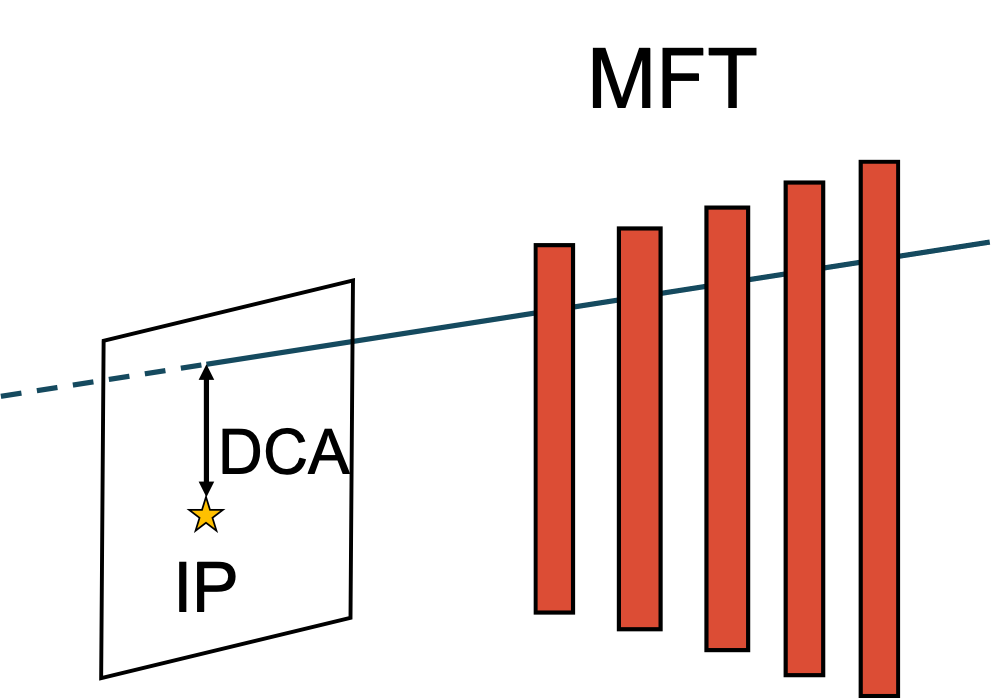
\includegraphics[keepaspectratio, scale=0.15]{fig/3_3_DCA.png} % Left image
                \caption{DCA}
                \label{Analysis:reco:DCA}
            \end{minipage}
            % Right figure
            \hspace{0.5cm}
            \begin{minipage}{0.45\textwidth}
                \centering
                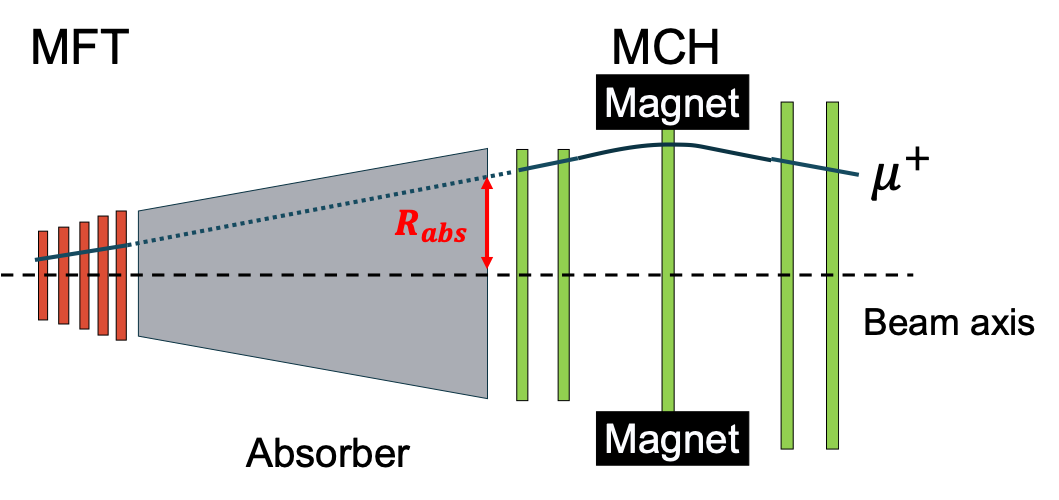
\includegraphics[keepaspectratio, scale=0.15]{fig/3_3_Rabs.png} % Right image
                \caption{$R_{abs}$}
                \label{Analysis:reco:R_abs}
            \end{minipage}
        \end{figure}

    \subsection{Single muon selection}
    \label{Single_muon_selection}
        The cuts applied to the obtained muon tracks are as follows:
        \begin{itemize}{}
            \item -3.6 <$\eta$ < -2.5
            \item 17.5 cm < $R_{abs}$ < 89.5 cm
            \item pDCA < 6$\sigma$
            \item MFT-MCH matching $\chi^2$ < 30
        \end{itemize}
        The $\eta$ cut is aligned with the MFT-MHC-MID acceptance. The $R_{abs}$ cut value is set to exclude values that are influenced by the presence of the hadron absorber rear end. The pDCA is the product of momentum and DCA, and this cut is applied to remove muons originating from beam gas. Tracks with pDCA larger than 6$\sigma$ when fitted with a Gaussian distribution are excluded. 
        The final MFT-MCH matching $\chi^2$ value is obtained from a fit using the detected points of the MFT and MCH tracks when matching them. The value used in this study is optimized, as described later, to maximize the statistical uncertainty of the yields for $\omega$ and $\phi$. 
    
        \subsection{Dimuon analysis}
        \label{Dimuon}
            \subsubsection{Dimuon reconstruction}
            \label{Dimuon_reco}
                Using the single muons selected in \ref{Single_muon_selection}, we reconstruct the dimuons. The mass, $p_T$, $\eta$, and $\phi$ of the dimuon are calculated as follows. First, we recalculate the $px$, $py$, $pz$, and $E$ from the single muon’s $p_T$, $\eta$, and $\phi$:
                \begin{eqnarray}
                    p_x &=& p_T \cos(\phi)\\
                    p_y &=& p_T \sin (\phi)\\
                    p_z &=& p_T \sinh (\eta)\\
                    E &=& \sqrt{p_T^2 \cosh^2(\eta) + m_\mu^2} 
                \end{eqnarray}
                Then, using the $px$, $py$, $pz$, and $E$ of the single muon, the $px$, $py$, $pz$, and $E$ of the dimuon are calculated. Using the resulting four-momentum of the dimuon, the pair’s $M_{\mu\mu}$, $p_T$, and $\eta$ are computed from the following equations:
                \begin{eqnarray}
                    M_{\mu\mu} &=& \sqrt{E^2 - (p_x^2 + p_y^2 + p_z^2)}\\
                    p_{T\mu\mu} &=& \sqrt{p_x^2 + p_y^2}\\
                    \eta_{\mu\mu} &=& -\log\left(\tan\left(\frac{1}{2}\arctan\left(\frac{\sqrt{p_x^2 + p_y^2}}{p_z}\right)\right)\right)
                \end{eqnarray}
                Using the above formulas, the physical quantities of the dimuon are calculated.
                The dimuon is formed by pairing opposite-charge muons within each event. If multiple combinations are possible, we pair all possible combinations and reconstruct the dimuon’s physical quantities. Since all possible combinations are considered, the mass distribution is also reconstructed for uncorrelated muon pairs. This is referred to as the combinatorial background. As will be described in the next section, this background can be statistically subtracted.
                
            \subsubsection{Combinatorial background subtraction}
            \label{Analysis:Dimuon:Combinatorial BG subtraction}
                Muons detected by the detector cannot be distinguished from which parent particle they originated. Therefore, when forming the muon pairs, all the $\mu^+$ and $\mu^-$ are paired within each collision event, and the mass is reconstructed. Then, the uncorrelated mass distribution is estimated and subtracted later. By doing so, the mass distribution of the correlated muon pairs can be obtained.
                In this study, the Like-sign method was used. The Like-sign method estimates the uncorrelated background events using the mass distribution of same-sign muon pairs obtained from the same event. The formula is as follows:
                \begin{eqnarray}
                    \dv{N_{sig}}{m} &=& \dv{N_{same}^{+-}}{m} - 2R \sqrt{\dv{N_{same}^{++}}{m} \dv{N_{same}^{--}}{m}}\\
                    2R &=& \frac{\dv{N_{mix}^{+-}}{m}}{\sqrt{\dv{N_{mix}^{++}}{m} \dv{N_{mix}^{--}}{m}}} 
                \end{eqnarray}
                where, $\dv{N_{sig}}{m}$ represents the number of correlated muons at each mass, $\dv{N_{same}^{**}}{m}$ represents the number of same-sign muon pairs in the same event (** corresponds to the muon sign), and $\dv{N_{mix}^{**}}{m}$ represents the number of muon pairs formed from different events. R is a term to correct for the acceptance difference due to the muon sign. If there is no acceptance difference due to the sign, R = 1. In this analysis, since muon pairs from different events were not combined, R = 1 was used for the calculation.
                The characteristic of the Like-sign method is that it subtracts uncorrelated background events using same-sign muon pairs from the same event. This allows for the subtraction of weakly correlated particles within each event, such as those caused by elliptic flow in heavy-ion collisions. The uncorrelated background events estimated by the Like-sign method depend on the $p_T$ of the dimuon. Therefore, the mass distributions were separated by the $p_T$ of the dimuon, and for each invariant mass distribution, the uncorrelated background events were subtracted using the Like-sign method. The resulting subtracted plots are shown in Figures \ref{Analysis:Dimuon:CB:CB_1to2} to \ref{Analysis:Dimuon:CB:CB_6to10}.
                \begin{figure}[htbp]
                    \centering
                    \begin{minipage}{0.45\textwidth}
                        \centering
                        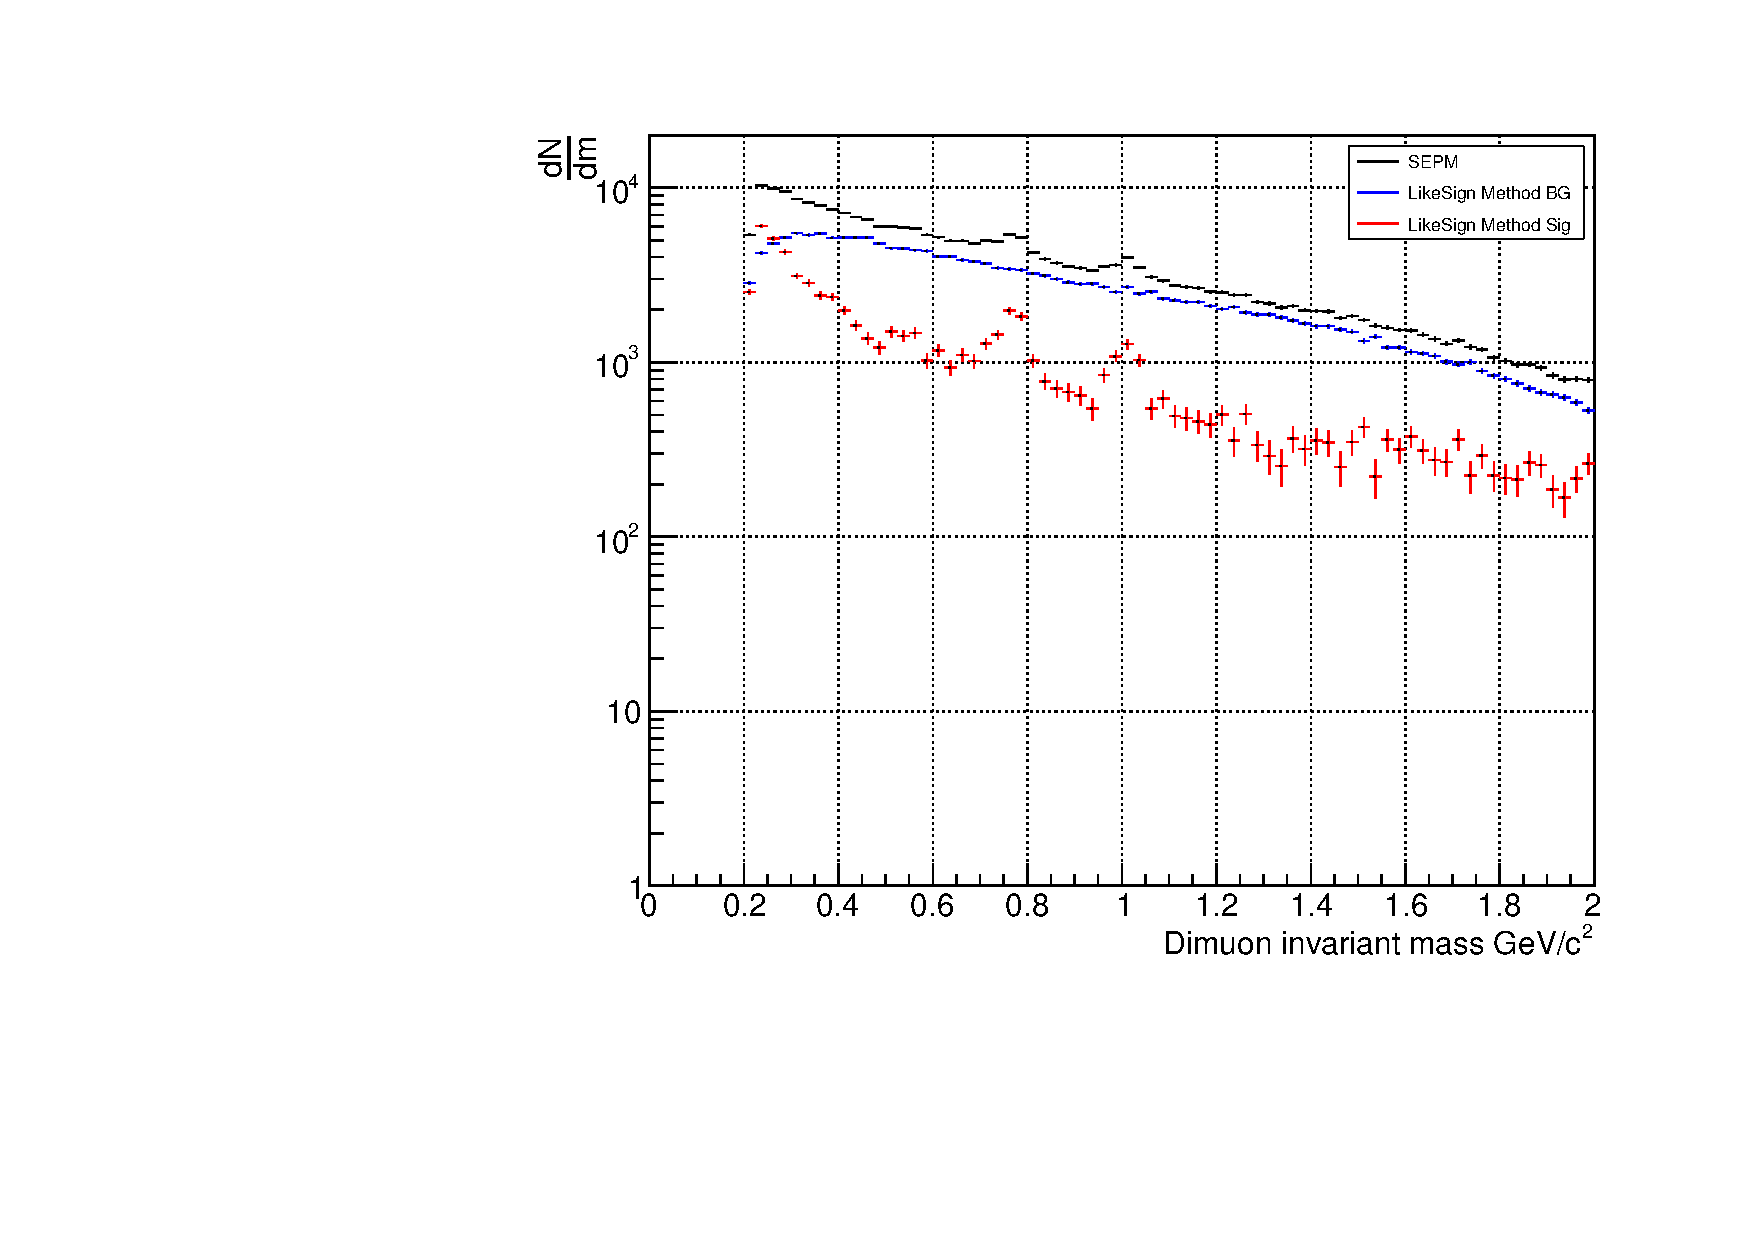
\includegraphics[width=\textwidth]{fig/3_4_1_CB_pt_1to2.pdf}
                        \captionsetup{labelformat=empty}
                        \caption{1 < $p_{T}$ < 2}
                        \label{Analysis:Dimuon:CB:CB_1to2}
                    \end{minipage}
                    \hfill
                    \begin{minipage}{0.45\textwidth}
                        \centering
                        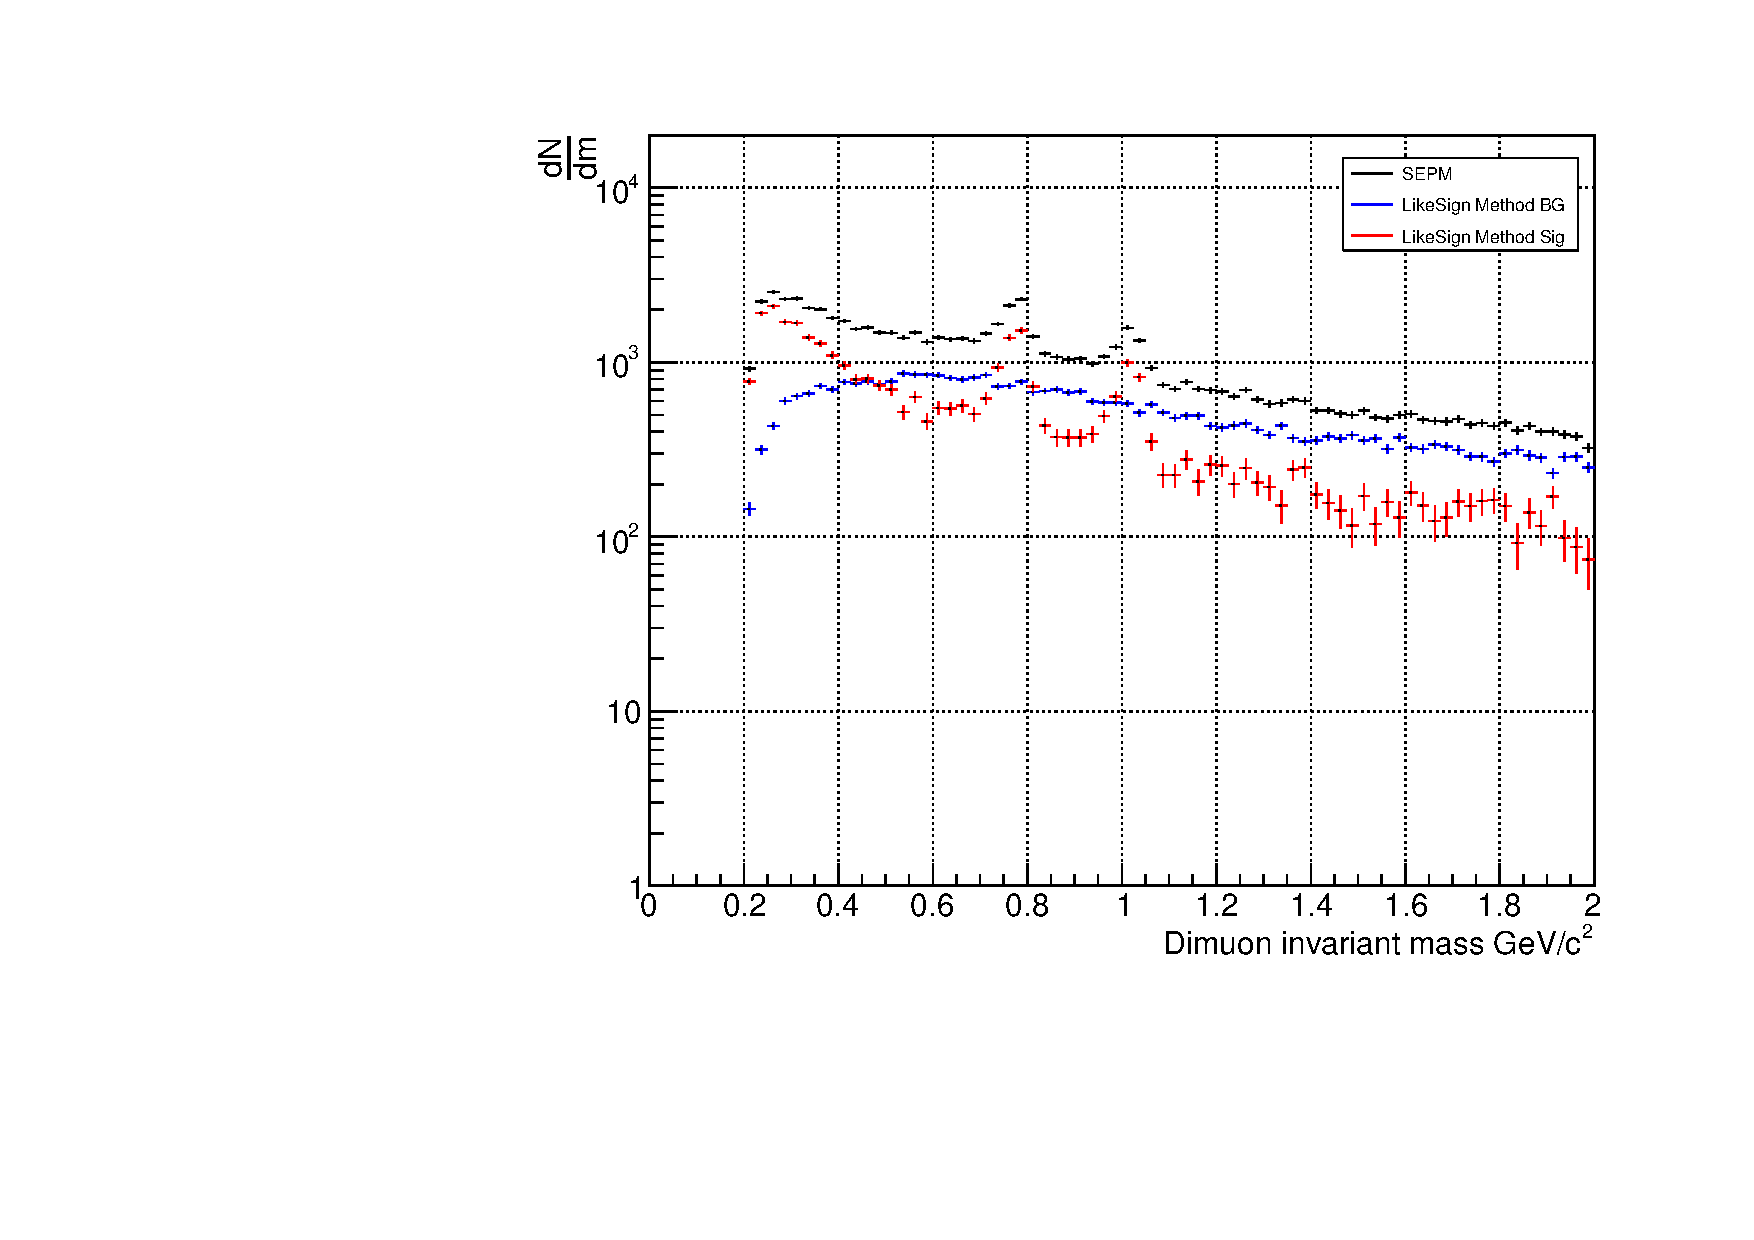
\includegraphics[width=\textwidth]{fig/3_4_1_CB_pt_2to3.pdf}
                        \captionsetup{labelformat=empty}
                        \caption{2 < $p_{T}$ < 3}
                        \label{Analysis:Dimuon:CB:CB_2to3}
                    \end{minipage}
                    \\
                    \vspace{1em}
                    \begin{minipage}{0.45\textwidth}
                        \centering
                        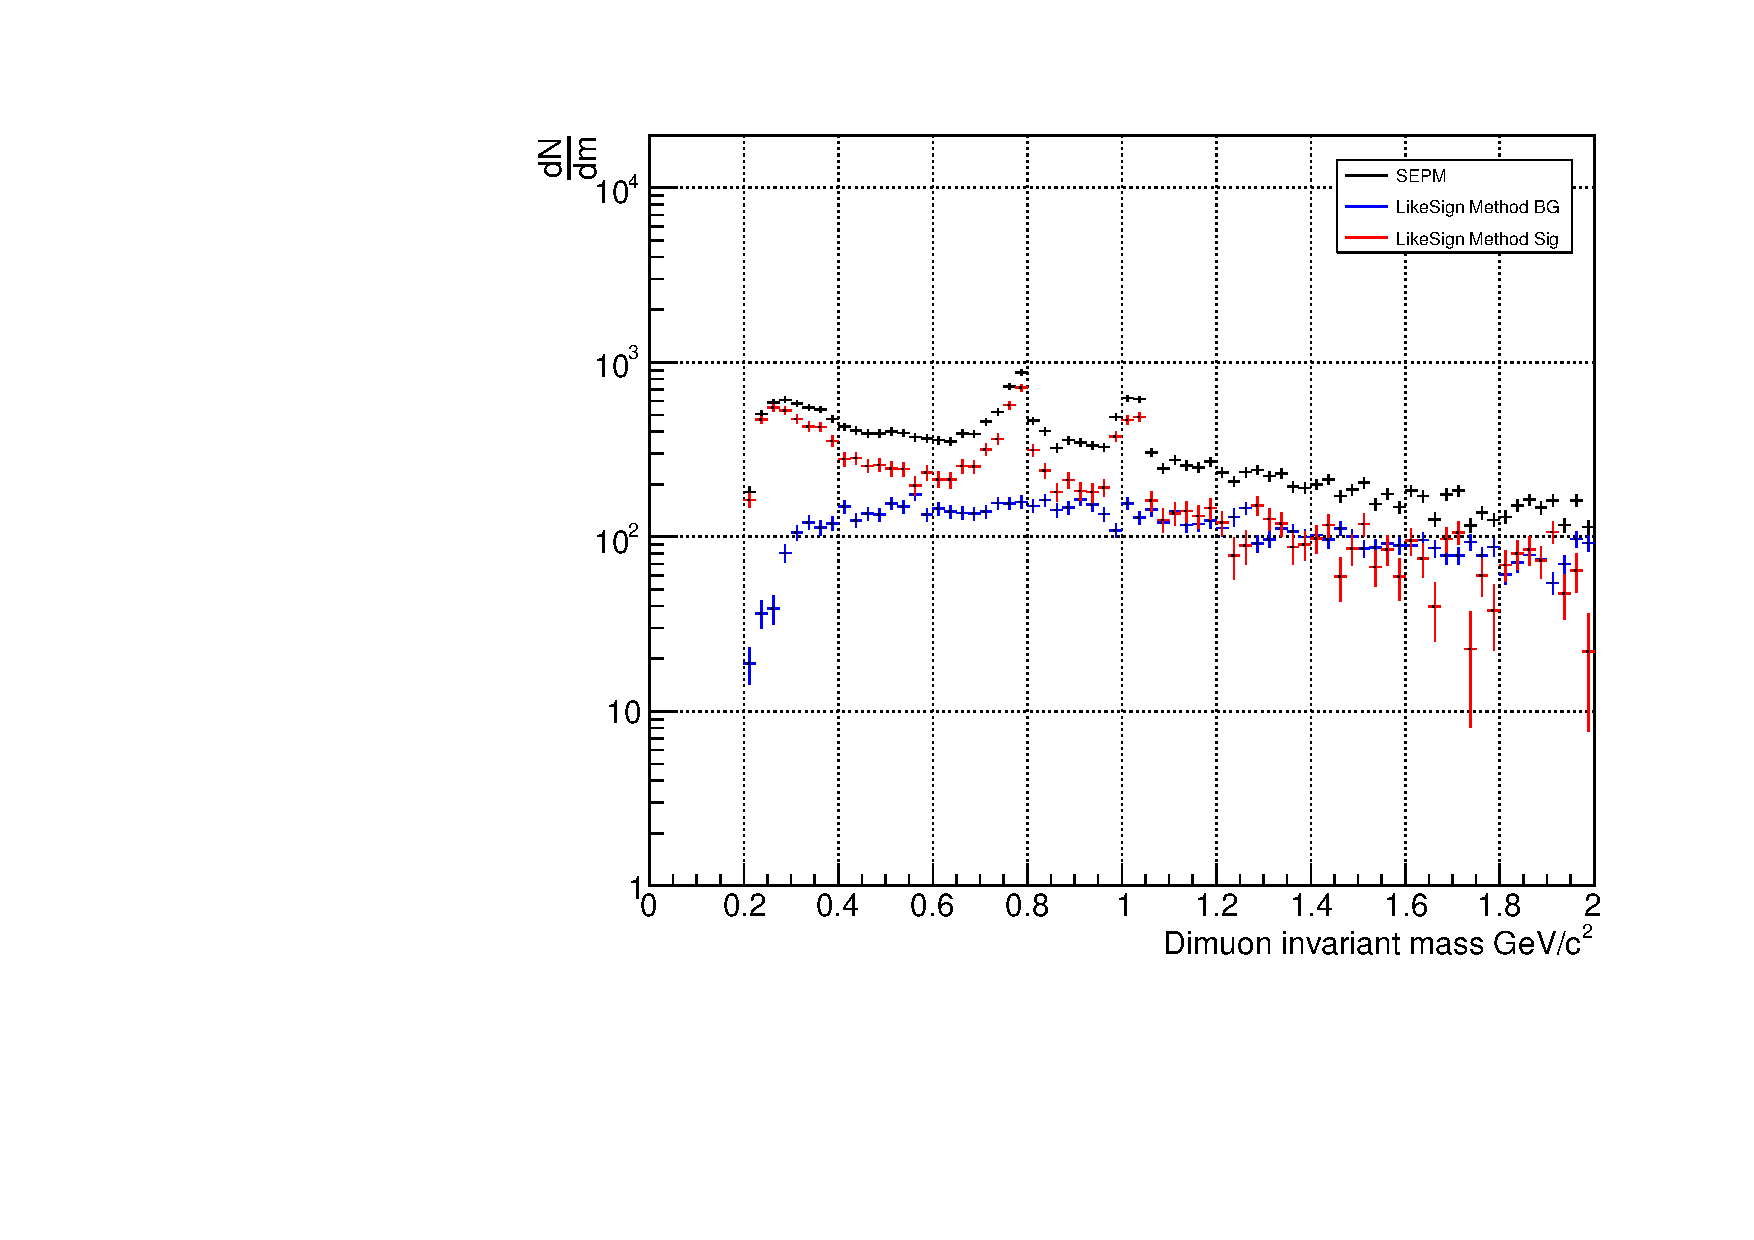
\includegraphics[width=\textwidth]{fig/3_4_1_CB_pt_3to4.pdf}
                        \captionsetup{labelformat=empty}
                        \caption{3 < $p_{T}$ < 4}
                        \label{Analysis:Dimuon:CB:CB_3to4}
                    \end{minipage}
                    \hfill
                    \begin{minipage}{0.45\textwidth}
                        \centering
                        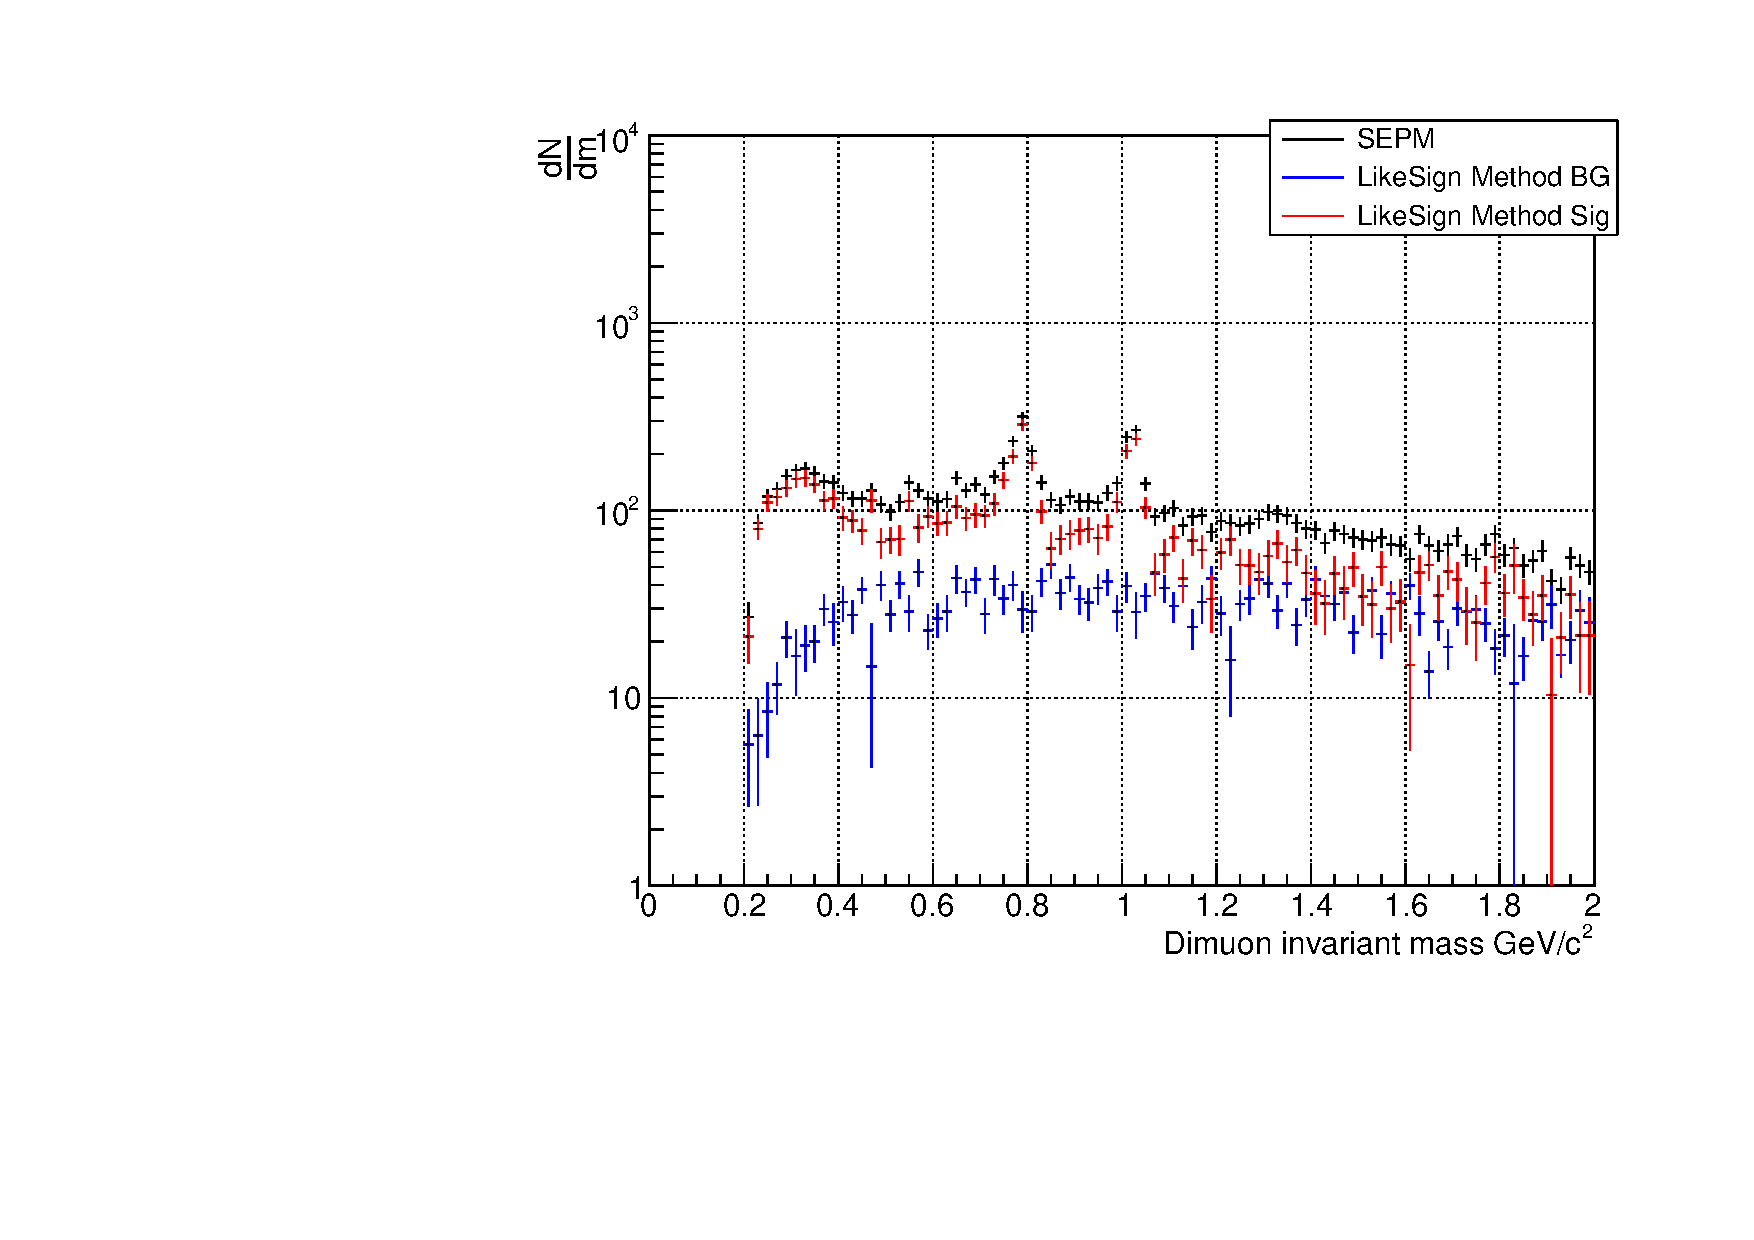
\includegraphics[width=\textwidth]{fig/3_4_1_CB_pt_4to5.pdf}
                        \captionsetup{labelformat=empty}
                        \caption{4 < $p_{T}$ < 5}
                        \label{Analysis:Dimuon:CB:CB_4to5}
                    \end{minipage}
                    \\
                    \vspace{1em}
                    \begin{minipage}{0.45\textwidth}
                        \centering
                        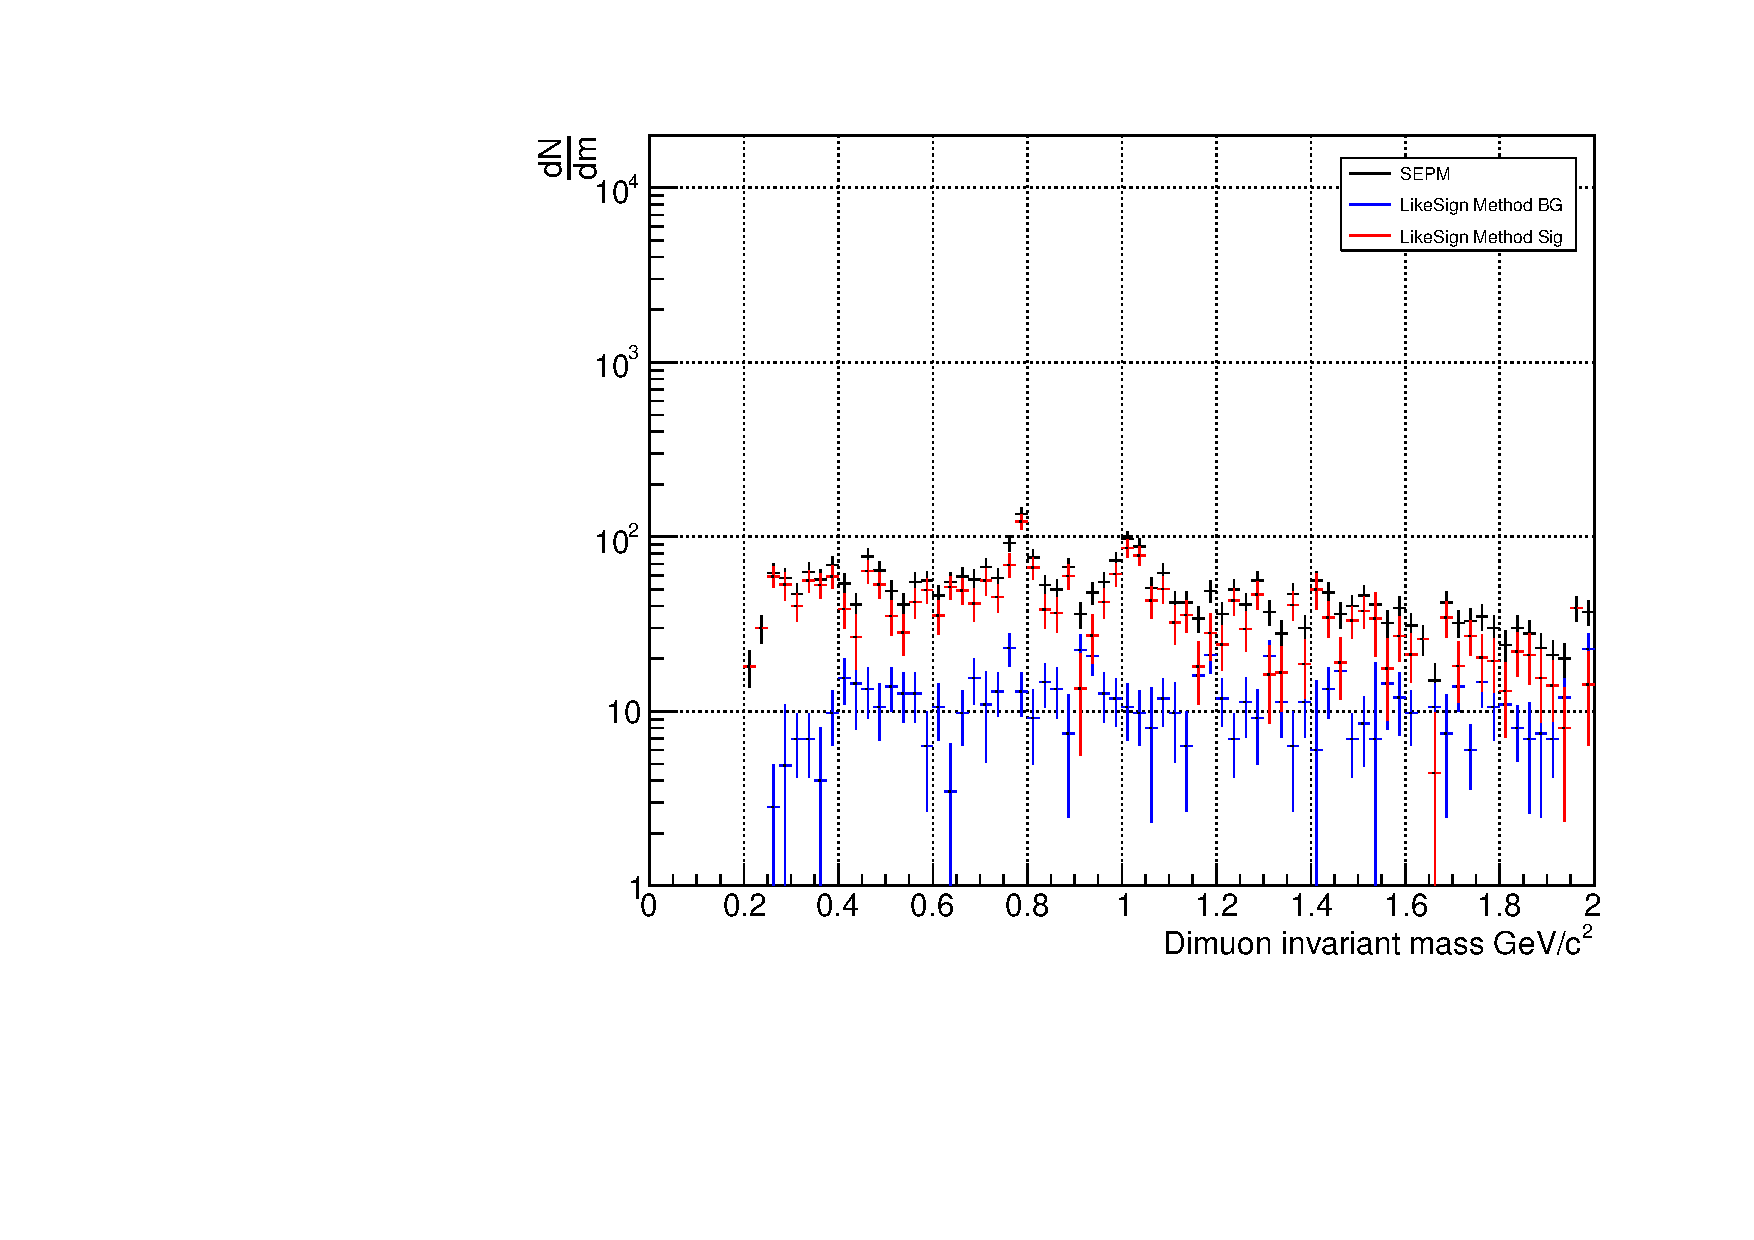
\includegraphics[width=\textwidth]{fig/3_4_1_CB_pt_5to6.pdf}
                        \captionsetup{labelformat=empty}
                        \caption{5 < $p_{T}$ < 6}
                        \label{Analysis:Dimuon:CB:CB_5to6}
                    \end{minipage}
                    \hfill
                    \begin{minipage}{0.45\textwidth}
                        \centering
                        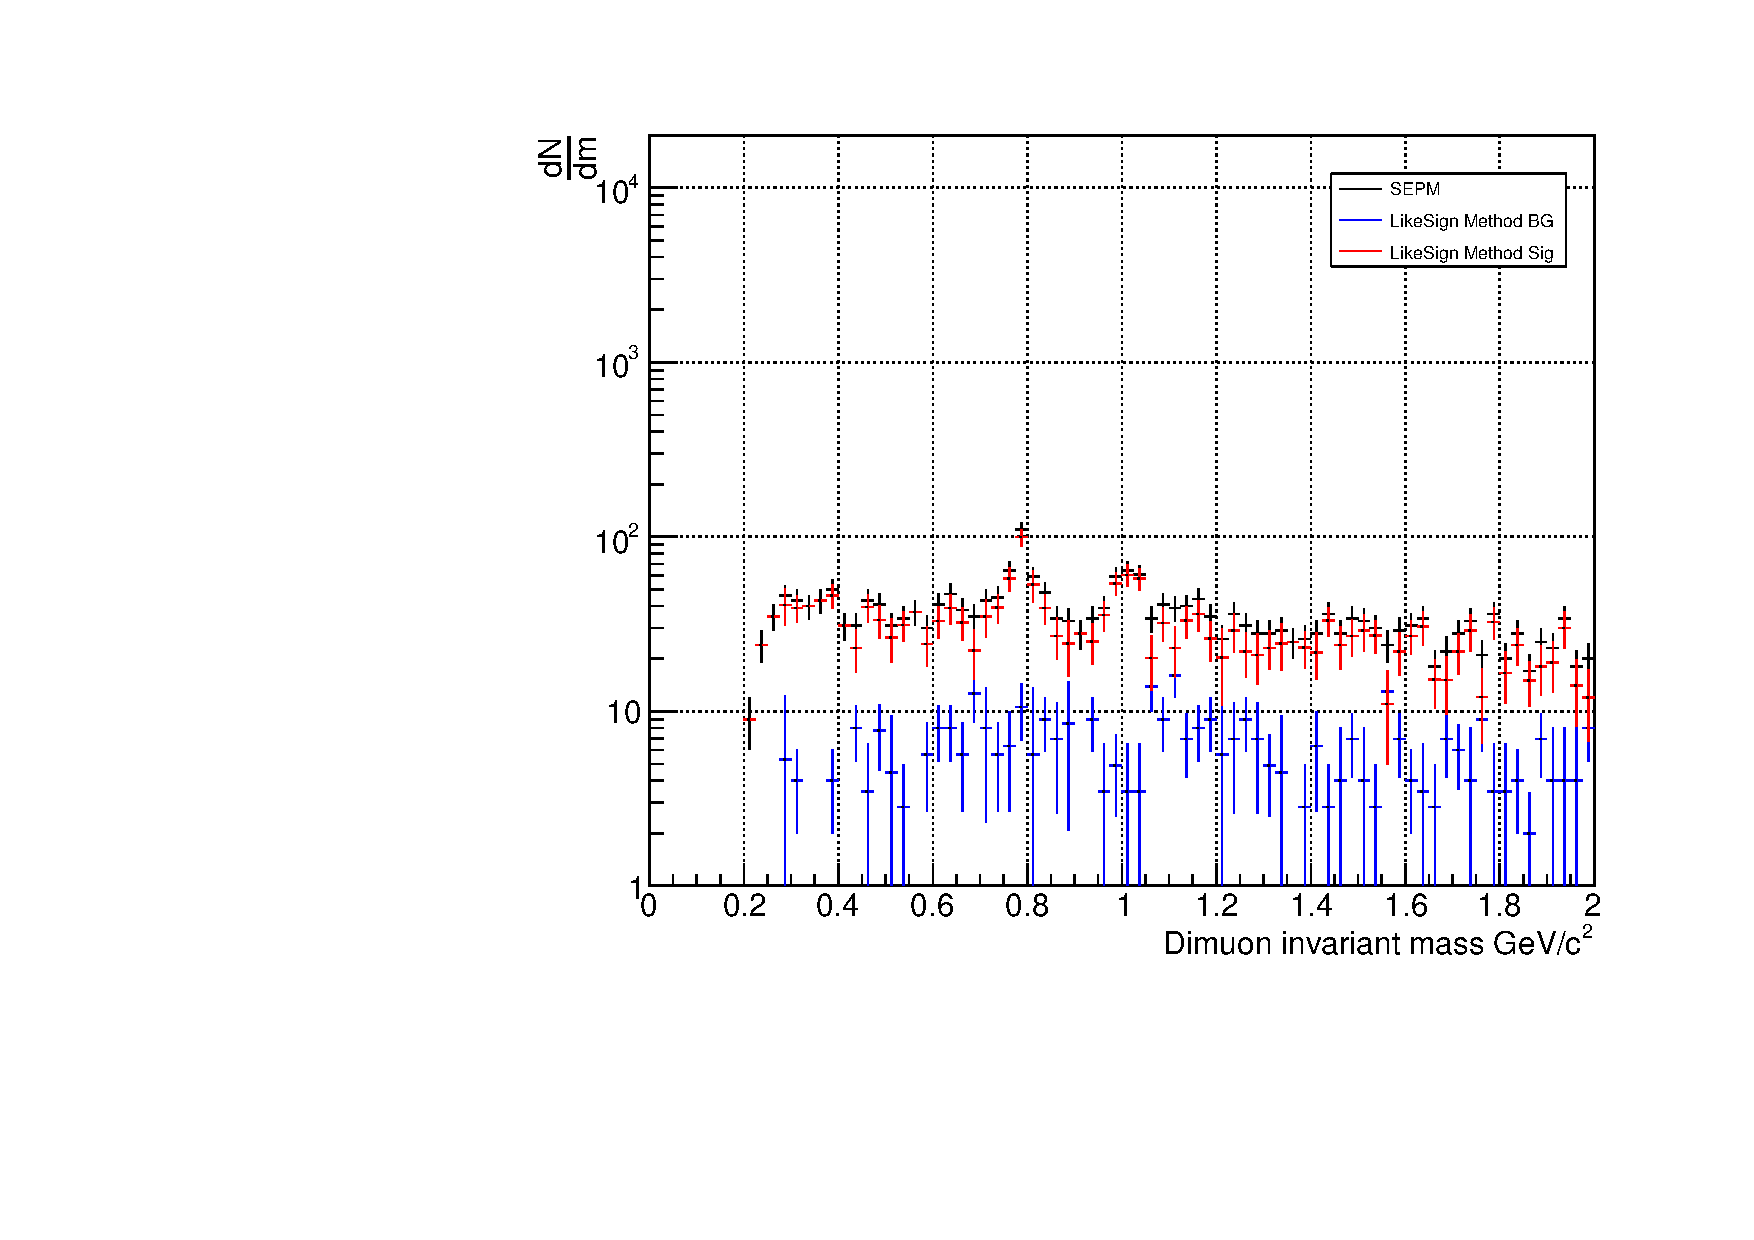
\includegraphics[width=\textwidth]{fig/3_4_1_CB_pt_6to10.pdf}
                        \captionsetup{labelformat=empty}
                        \caption{6 < $p_{T}$ < 10}
                        \label{Analysis:Dimuon:CB:CB_6to10}
                    \end{minipage}
                    \caption{Results after subtracting uncorrelated background events in each $p_T$ region}
                    \label{Analysis:Dimuon:CB:CB_pt_separation}
                \end{figure}
                The black line represents the distribution obtained by pairing muons with opposite charges within the same event and reconstructing the mass. The blue line represents the estimated uncorrelated background events using the Like-sign method. The red line represents the distribution obtained by subtracting the blue distribution from the black distribution, which corresponds to the correlated dimuon invariant mass distribution. In the $0 < p_T < 1$(GeV) region, the MFT-MCH matching quality was insufficient, and no peaks for $\omega$ and $\phi$ were observed. The $6 < p_T < 10$(GeV) region was taken wider than other transverse momentum regions to preserve the statistical significance.
        
            \subsubsection{Peak extraction of $\omega \rightarrow \mu\mu ,\phi \rightarrow \mu\mu$}
            \label{Peak_extraction}
                The distributions of the correlated dimuon invariant mass obtained from \ref{Analysis:Dimuon:Combinatorial BG subtraction} are used to extract the distributions of $\omega \rightarrow \mu\mu,\phi \rightarrow \mu\mu$. The dimuon invariant mass distribution under 2(GeV) contains pairs of muons coming from light mesons and open HF:
                \begin{itemize}
                    \item $\eta \rightarrow \mu^+ \mu^-$
                    \item $\eta \rightarrow \mu^+ \mu^- \gamma$
                    \item $\rho \rightarrow \mu^+ \mu^-$
                    \item $\omega \rightarrow \mu^+ \mu^-$
                    \item $\omega \rightarrow \mu^+ \mu^- \pi^0$
                    \item $\eta' \rightarrow \mu^+ \mu^- \gamma$
                    \item $\phi \rightarrow \mu^+ \mu^-$
                    \item $c\bar{c} \rightarrow D\bar{D} \rightarrow \mu^+ \mu^- + others$
                    \item $b\bar{b} \rightarrow B\bar{B} \rightarrow \mu^+ \mu^- + others$
                \end{itemize}
                The $\omega \rightarrow \mu\mu,\phi \rightarrow \mu\mu$ processes each have sharp peak structures with peaks around 0.8GeV and 1.0GeV in the mass distribution. In this analysis, all distributions other than these are considered background events. Therefore, an exponential fit is performed to the continuous component of the mass distribution, and only the peaks are extracted. The fit function is as follows:
                \begin{eqnarray}
                    f(m)=N_0*\exp{-p1* m}+N_{\omega}*\exp{-\frac{1}{2}\qty(\frac{m-M_{\omega}}{\sigma_{\omega}})^2}+N_{\phi}*\exp{-\frac{1}{2}\qty(\frac{m-M_{\phi}}{\sigma_{\phi}})^2}
                \end{eqnarray}
                where, $N_0, N_{\omega}, N_{\phi}, M_{\omega}, M_{\phi}, \sigma_{\omega}, \sigma_{\phi}$ are fit parameters, with $M_{\omega}$ and $M_{\phi}$ representing the mean mass positions of $\omega$ and $\phi$, and $\sigma_{\omega}$ and $\sigma_{\phi}$ corresponding to the mass widths. This fit function was applied to the correlated invariant mass distributions in \ref{Analysis:Dimuon:CB:CB_1to2} ~ \ref{Analysis:Dimuon:CB:CB_6to10}. The results are shown in \ref{Analysis:Dimuon:Yield:fit_1to2} ~ \ref{Analysis:Dimuon:Yield:fit_6to10}.\@
                \begin{figure}[htbp]
                    \centering
                    \begin{minipage}{0.45\textwidth}
                        \centering
                        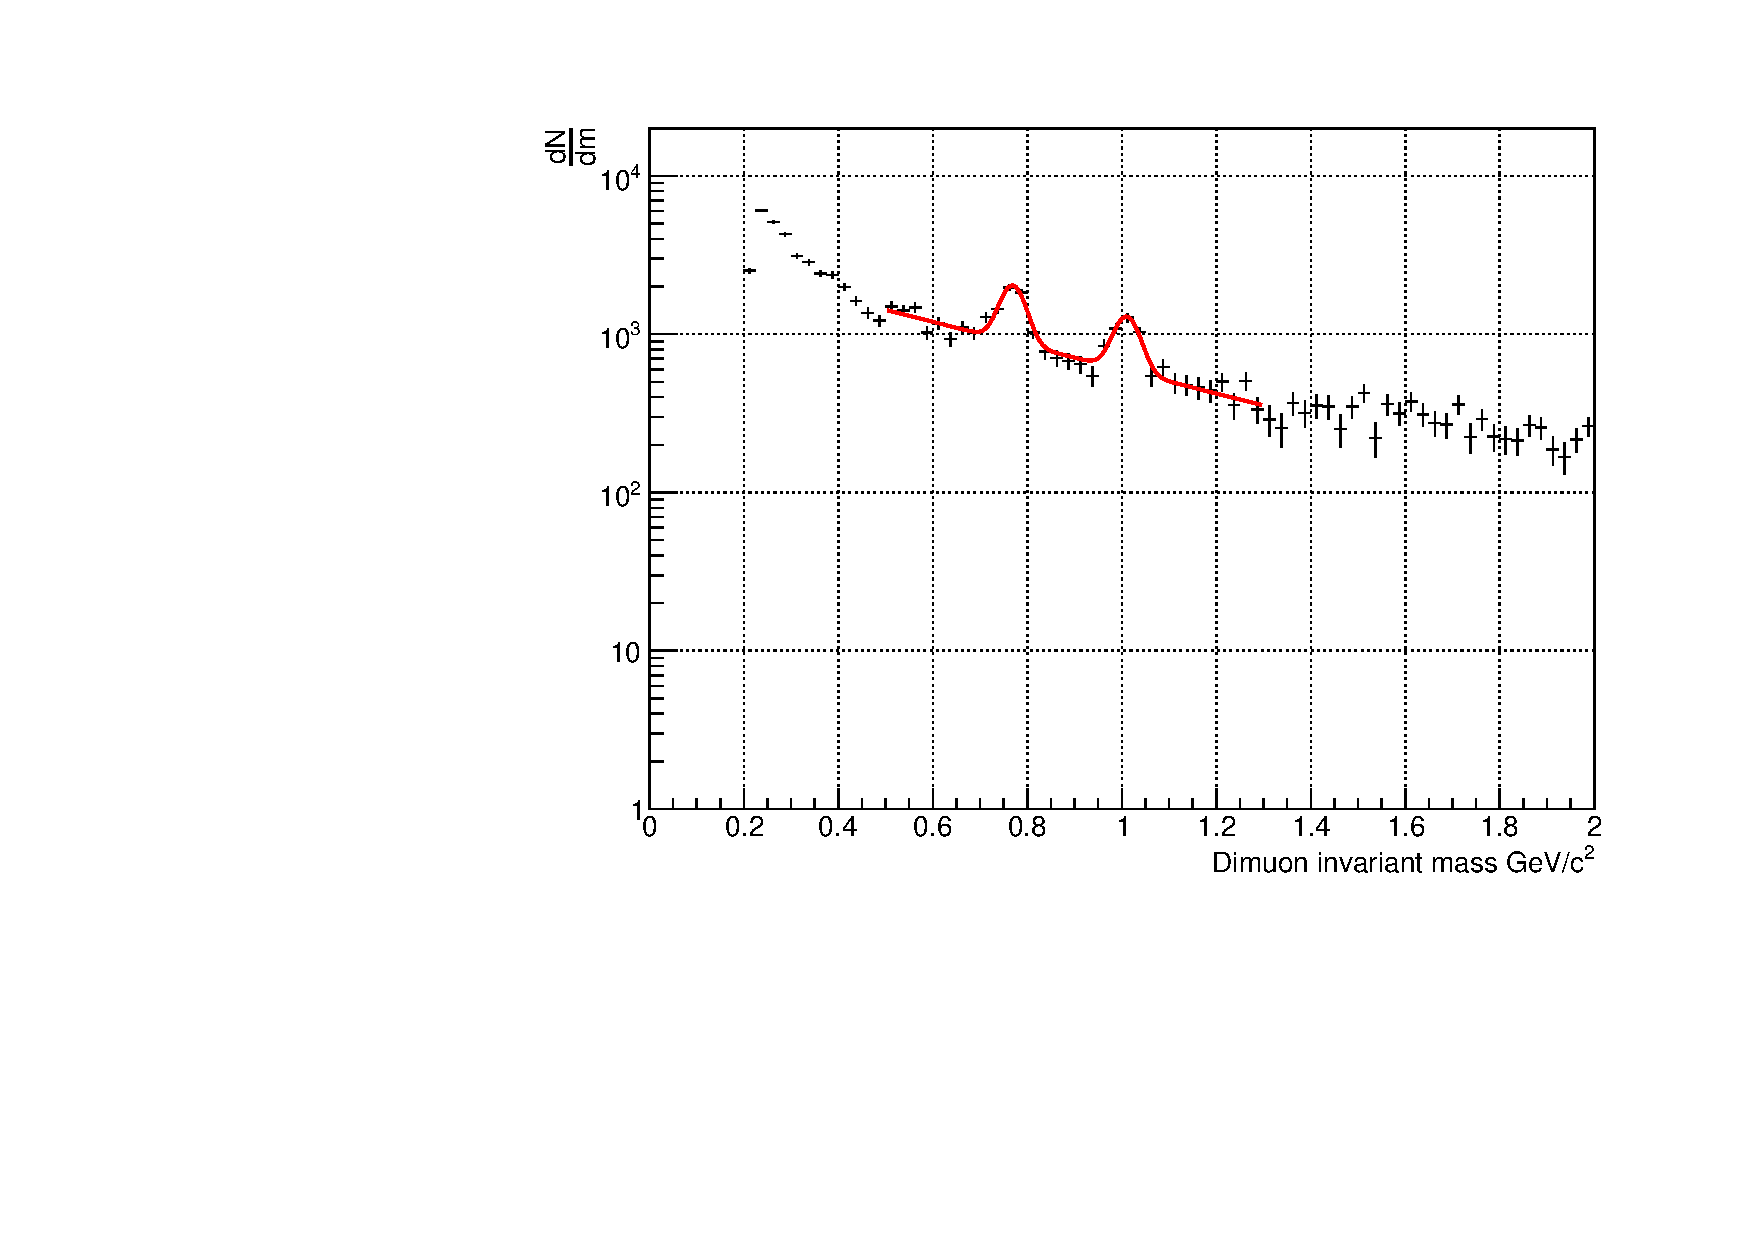
\includegraphics[width=\textwidth]{fig/3_4_2_fit_pt_1to2.pdf}
                        \captionsetup{labelformat=empty}
                        \caption{1 < $p_{T}$ < 2}
                        \label{Analysis:Dimuon:Yield:fit_1to2}
                    \end{minipage}
                    \hfill
                    \begin{minipage}{0.45\textwidth}
                        \centering
                        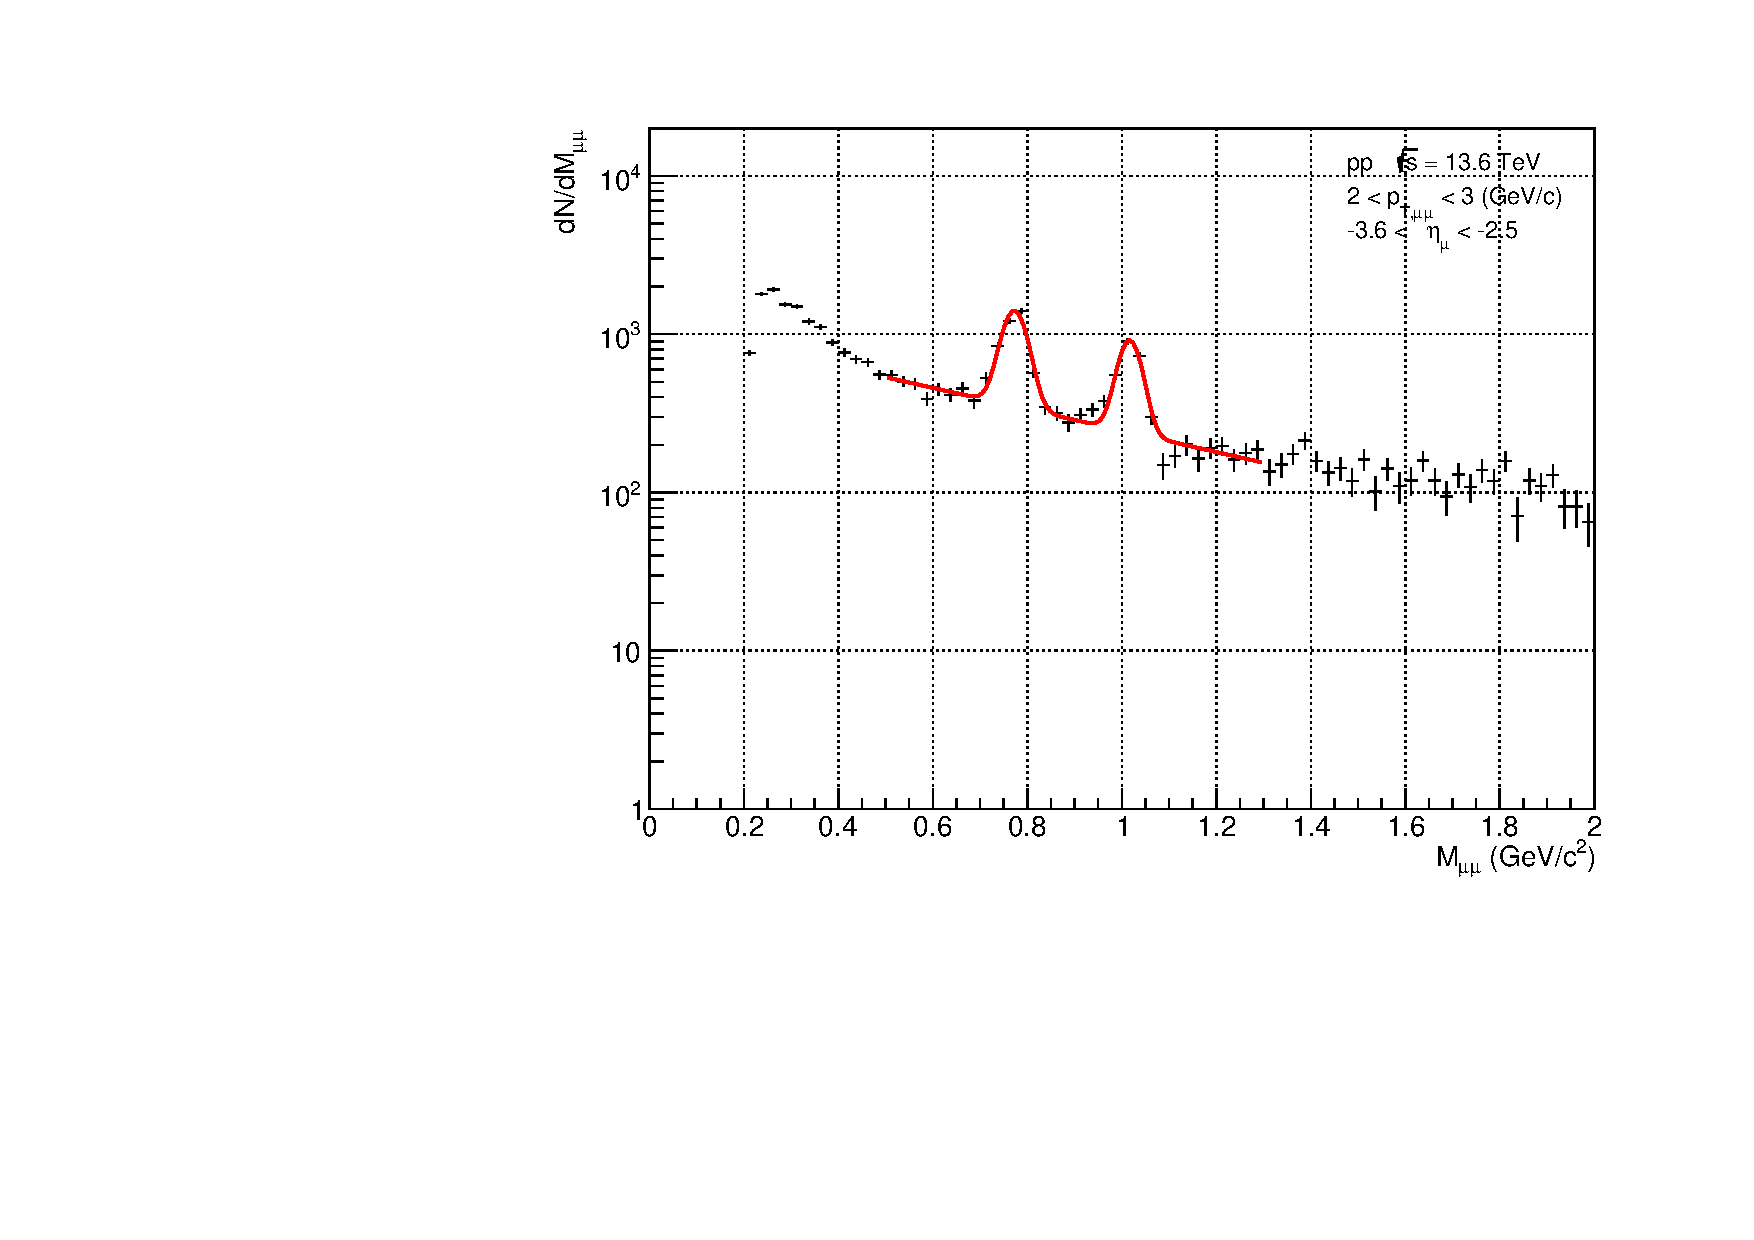
\includegraphics[width=\textwidth]{fig/3_4_2_fit_pt_2to3.pdf}
                        \captionsetup{labelformat=empty}
                        \caption{2 < $p_{T}$ < 3}
                        \label{Analysis:Dimuon:Yield:fit_2to3}
                    \end{minipage}
                    \\
                    \vspace{1em}
                    \begin{minipage}{0.45\textwidth}
                        \centering
                        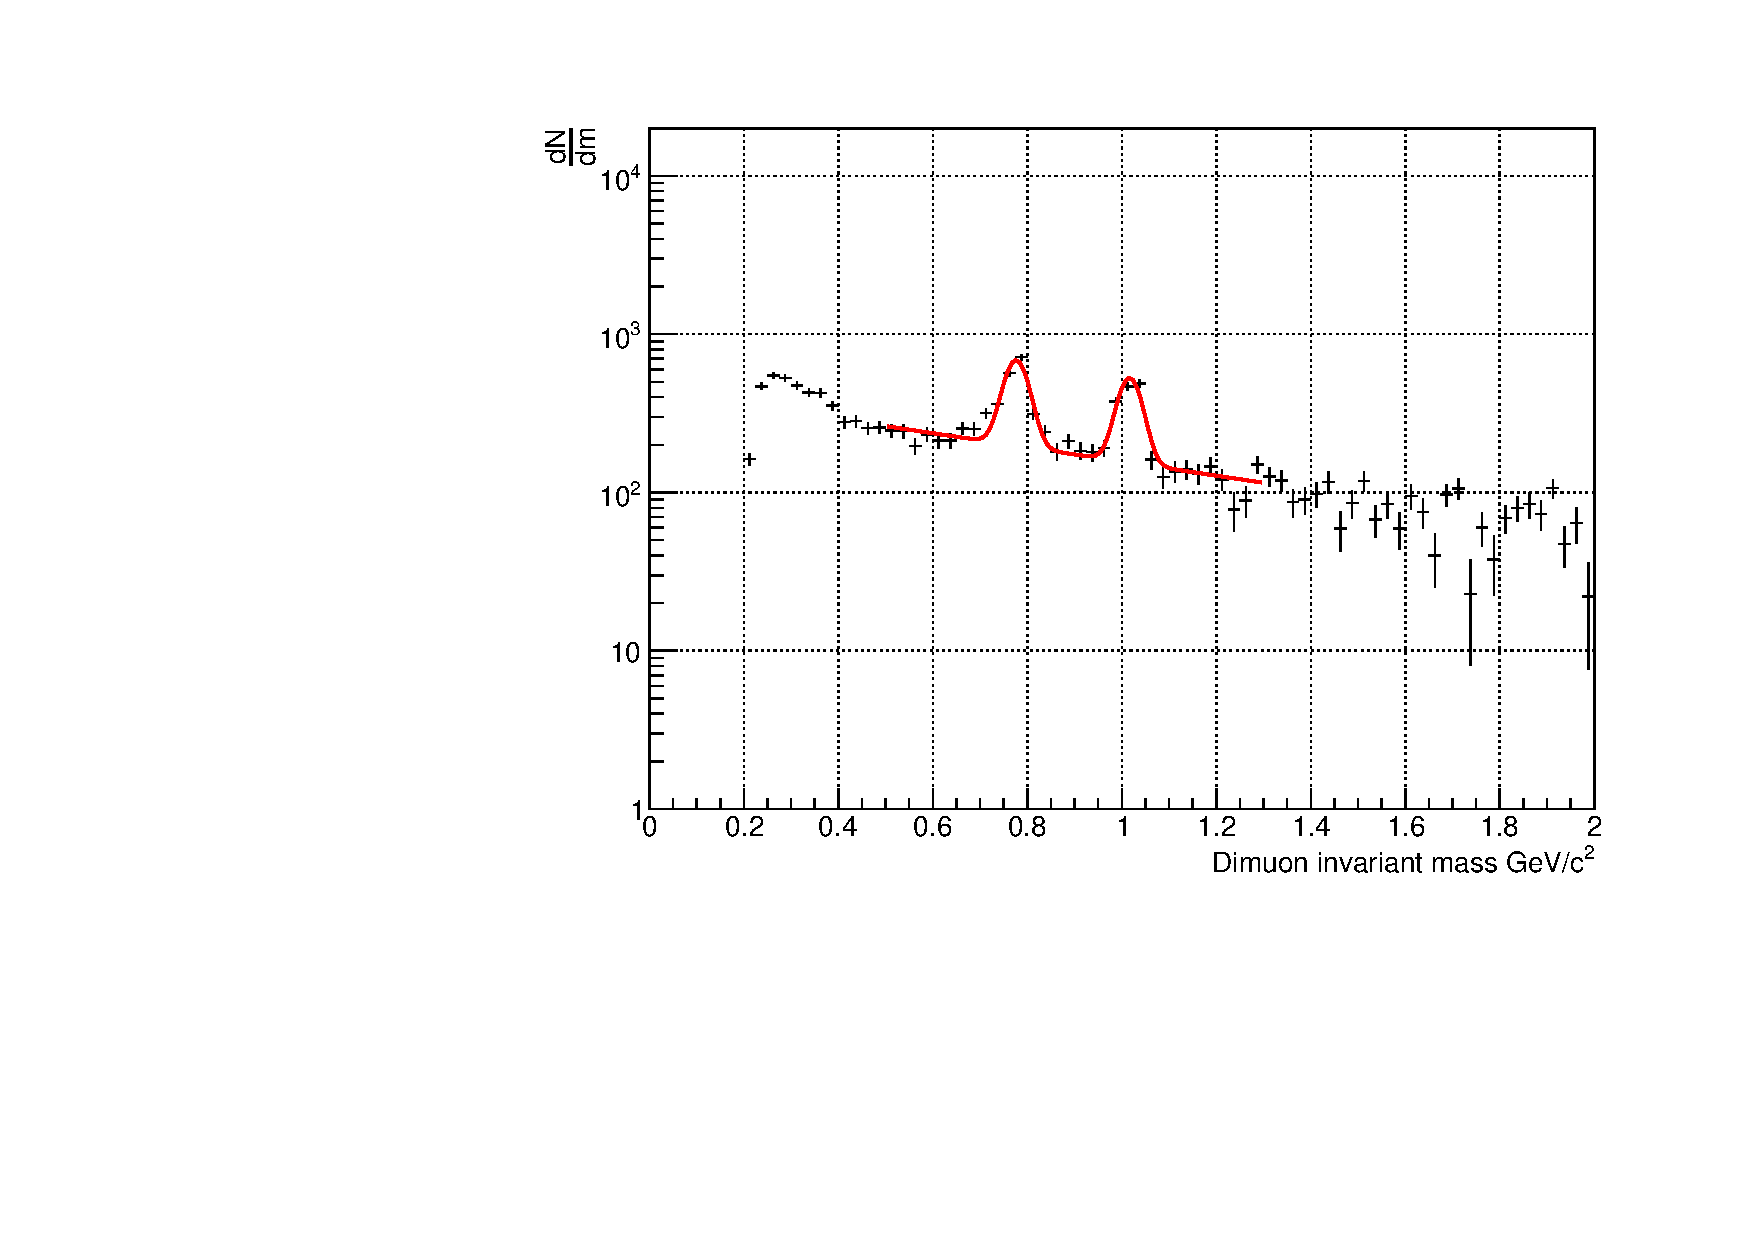
\includegraphics[width=\textwidth]{fig/3_4_2_fit_pt_3to4.pdf}
                        \captionsetup{labelformat=empty}
                        \caption{3 < $p_{T}$ < 4}
                        \label{Analysis:Dimuon:Yield:fit_3to4}
                    \end{minipage}
                    \hfill
                    \begin{minipage}{0.45\textwidth}
                        \centering
                        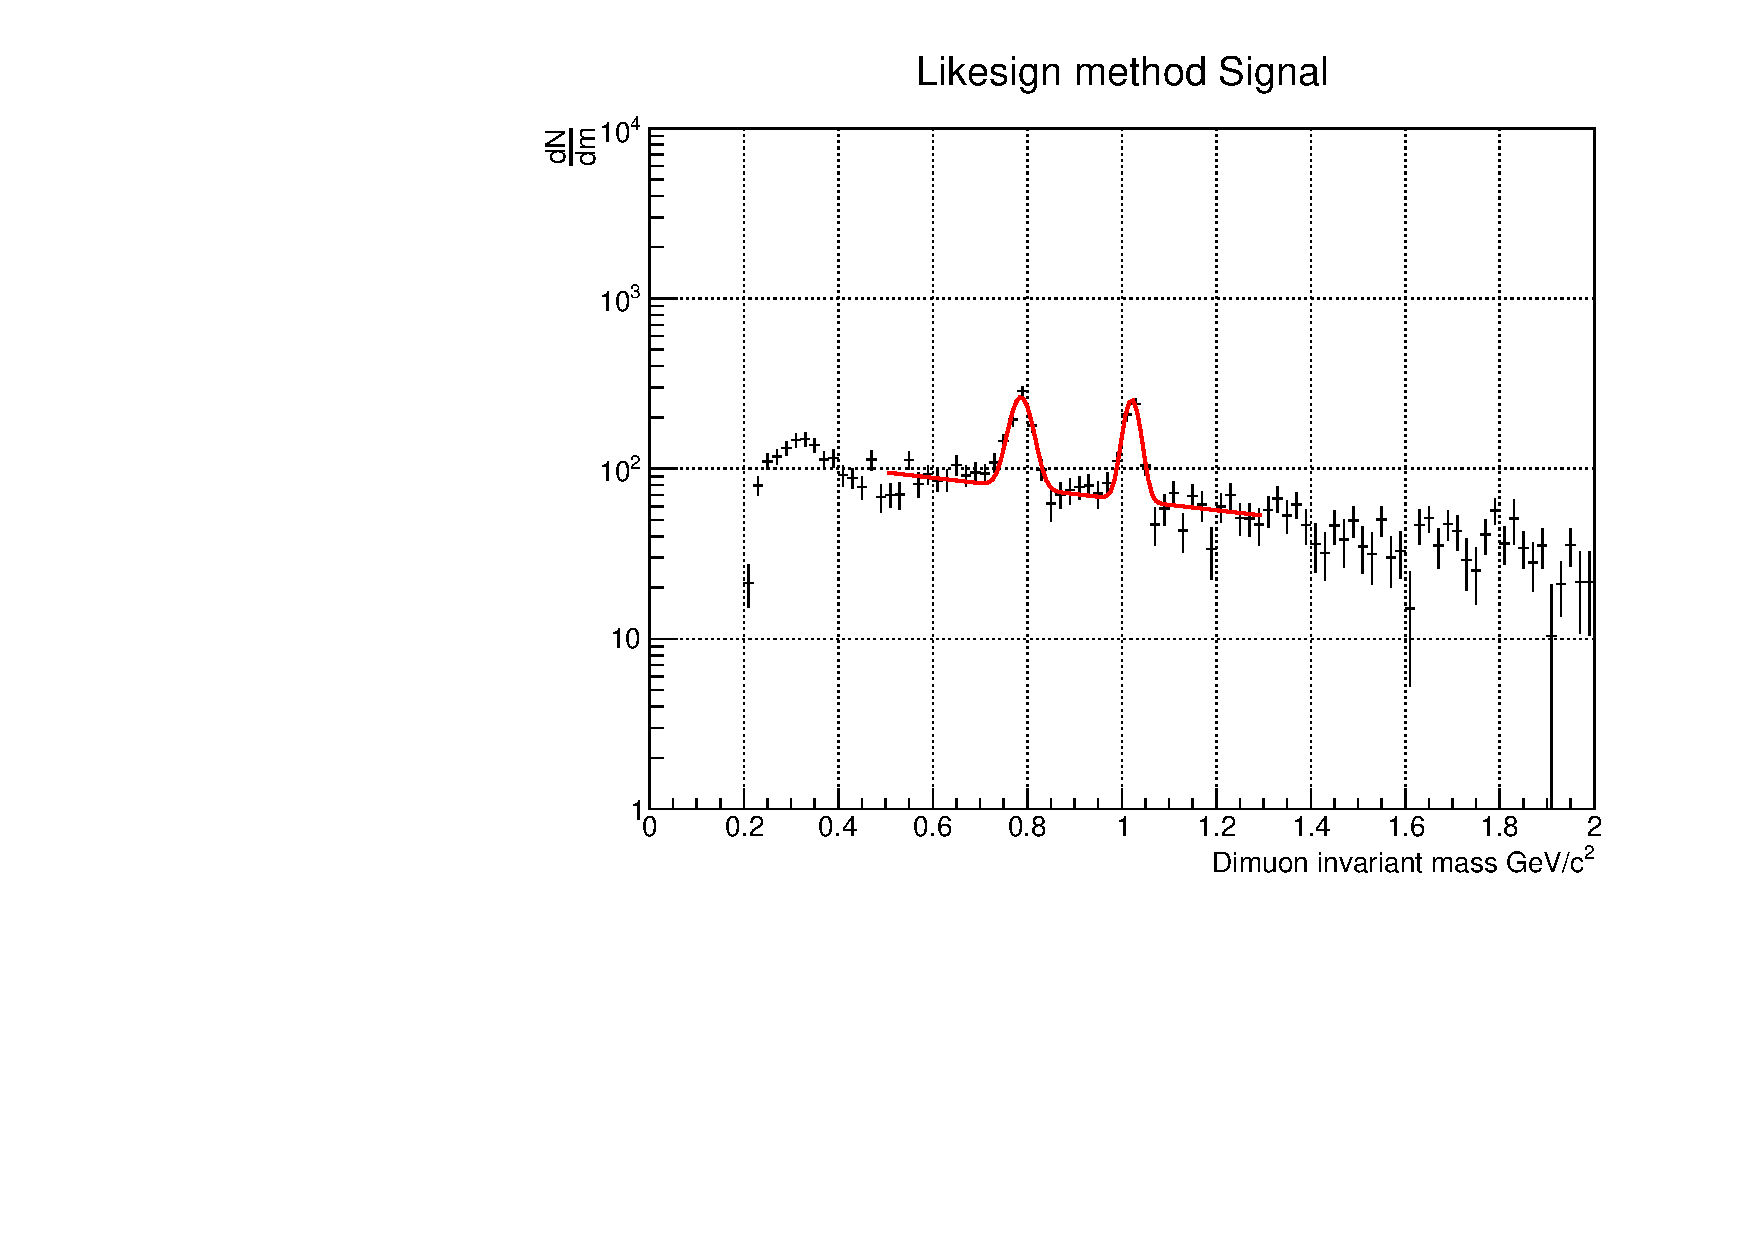
\includegraphics[width=\textwidth]{fig/3_4_2_fit_pt_4to5.pdf}
                        \captionsetup{labelformat=empty}
                        \caption{4 < $p_{T}$ < 5} 
                        \label{Analysis:Dimuon:Yield:fit_4to5}
                    \end{minipage}
                    \\
                    \vspace{1em}
                    \begin{minipage}{0.45\textwidth}
                        \centering
                        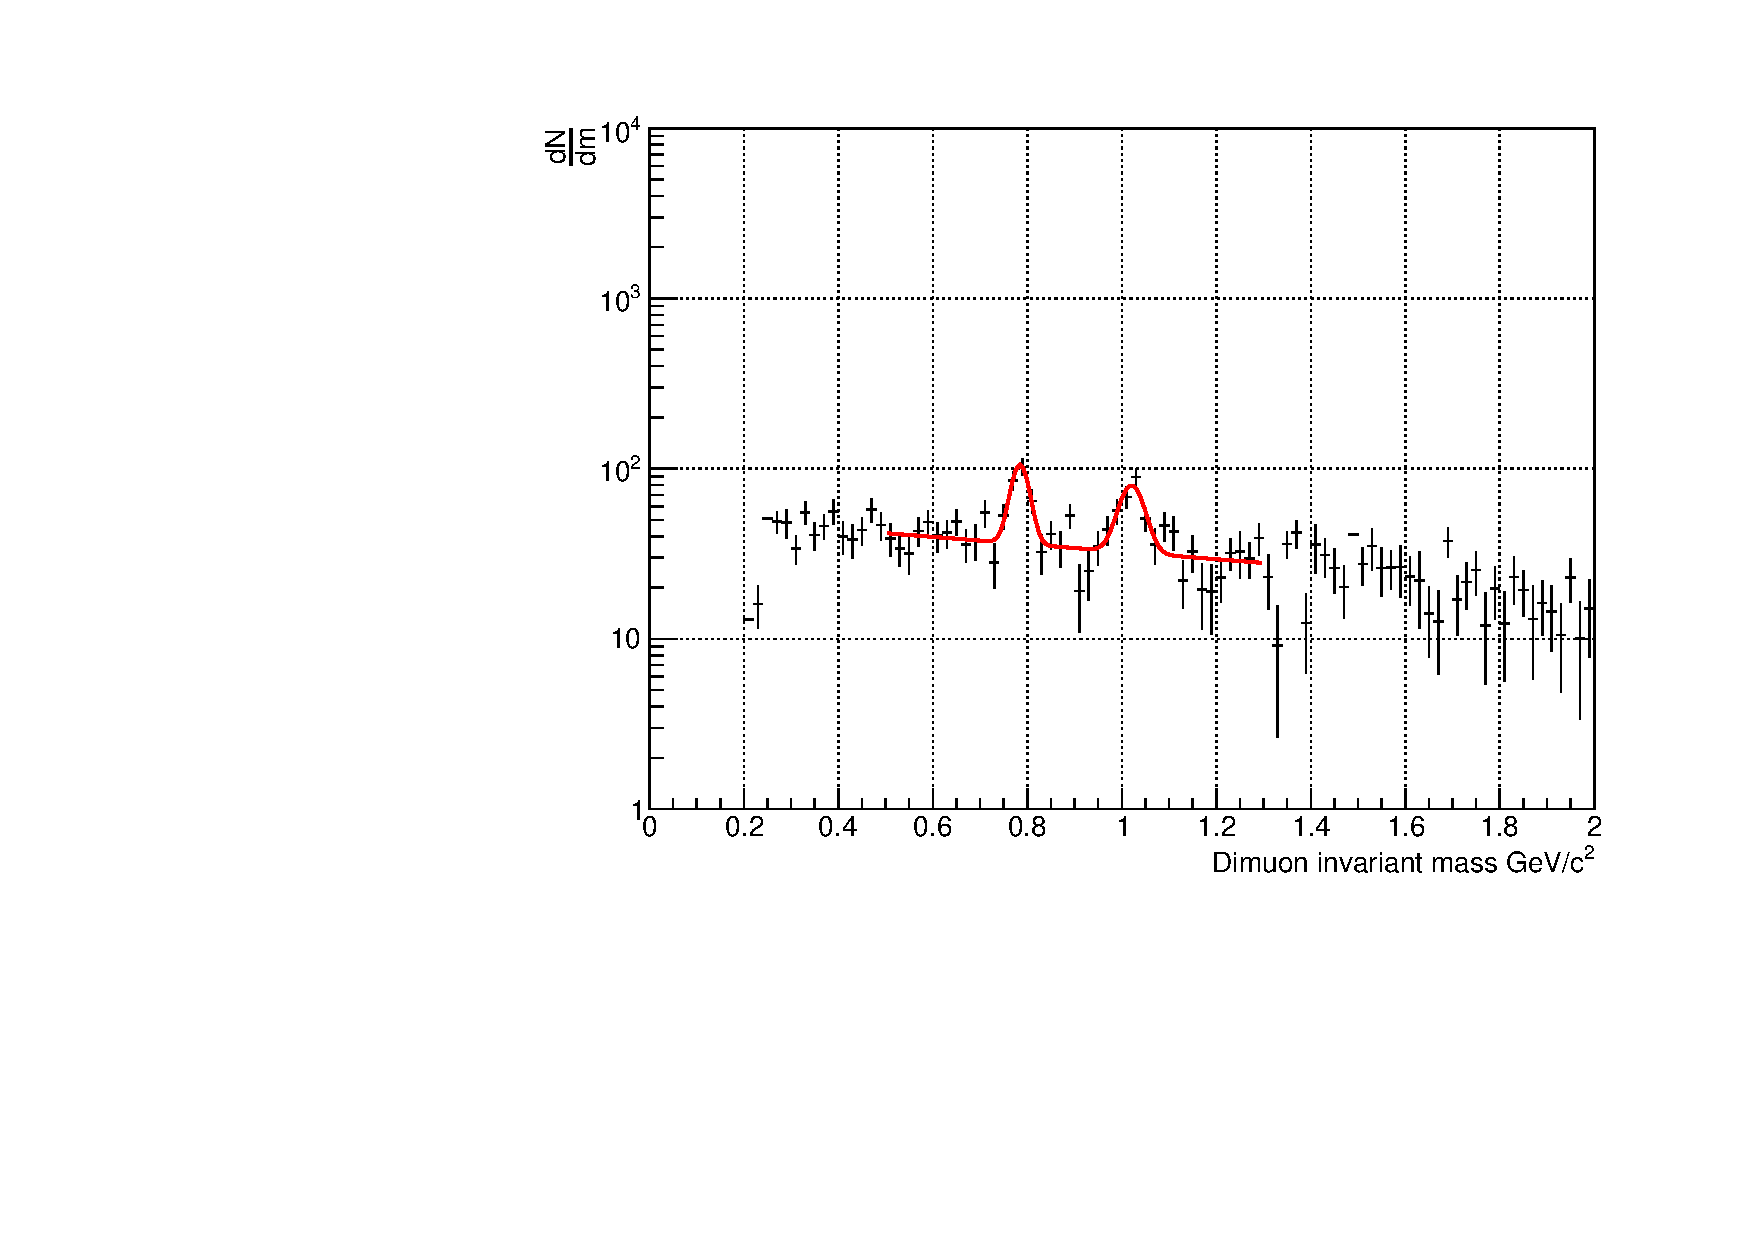
\includegraphics[width=\textwidth]{fig/3_4_2_fit_pt_5to6.pdf}
                        \captionsetup{labelformat=empty}
                        \caption{5 < $p_{T}$ < 6}
                        \label{Analysis:Dimuon:Yield:fit_5to6}
                    \end{minipage}
                    \hfill
                    \begin{minipage}{0.45\textwidth}
                        \centering
                        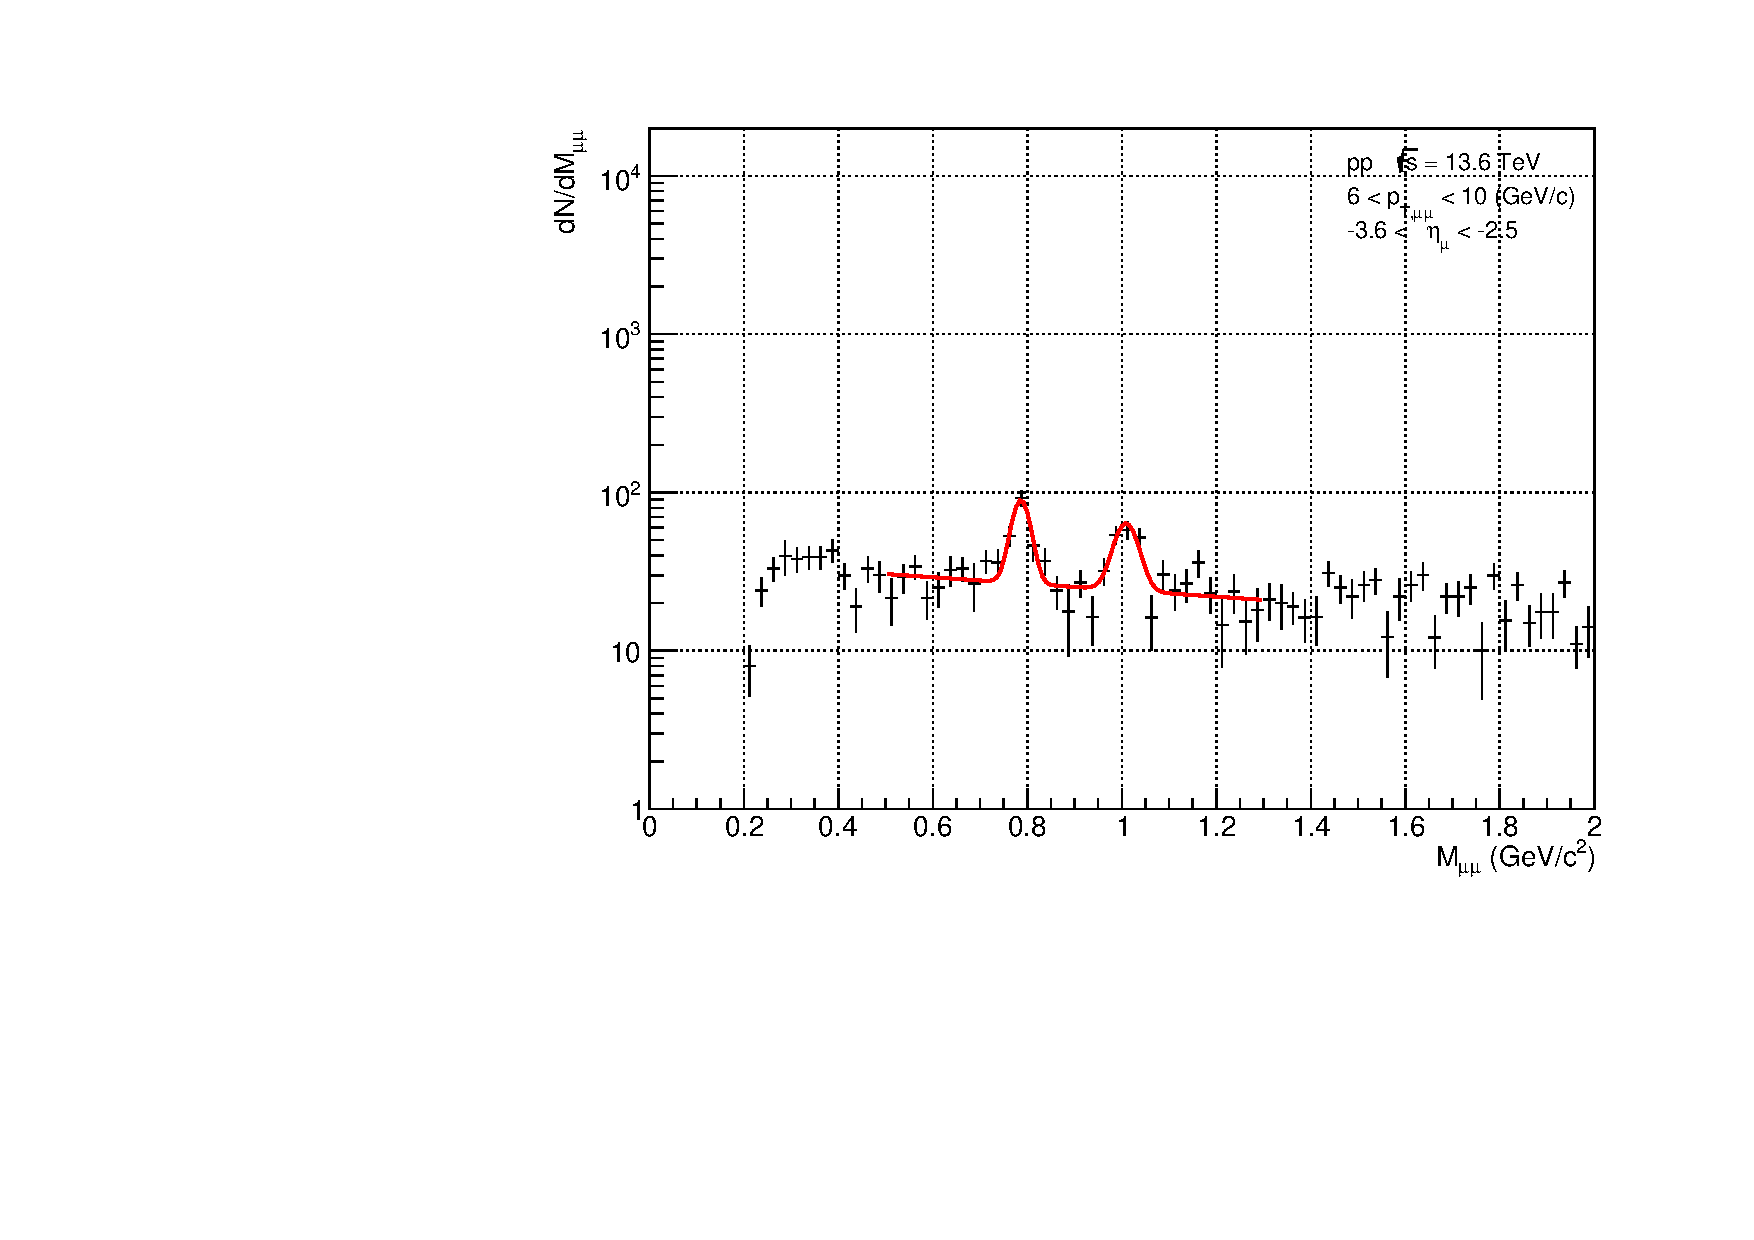
\includegraphics[width=\textwidth]{fig/3_4_2_fit_pt_6to10.pdf}
                        \captionsetup{labelformat=empty}
                        \caption{6 < $p_{T}$ < 10}
                        \label{Analysis:Dimuon:Yield:fit_6to10}
                    \end{minipage}
                    \caption{Results after subtracting uncorrelated background events in each momentum region.}
                \end{figure}
                The mean mass positions and mass widths for $\omega$ and $\phi$, as well as the fit $\chi^2$ values for each transverse momentum region, are summarized in the following table.
                    \begin{table}[htbp]
                        \centering
                        \caption{Fit Results}
                        \begin{tabular}{|c||c|c|c|c|c|}
                            \hline
                            & $\omega$ mean mass & $\omega$ mass width & $\phi$ mean mass & $\phi$ mass width & fit $\chi^2$ \\ \hline \hline
                            1 < $p_{T}$ < 2 &$0.771\pm0.002$& $0.024\pm0.002$ &$1.012\pm0.003$ &$0.027\pm 0.003$ & 52.34/32\\ \hline
                            2 < $p_{T}$ < 3 &$0.775\pm0.001$&$0.026\pm0.001$ & $1.017\pm0.002$& $0.024\pm 0.002$ & 42.07/32\\ \hline
                            3 < $p_{T}$ < 4 &$0.777\pm0.002$& $0.024\pm0.002$ &$1.018\pm0.002$ &$0.023\pm 0.001$ & 111.8/32\\ \hline
                            4 < $p_{T}$ < 5 &$0.788\pm0.002$& $0.022\pm0.002$ &$1.02\pm0.00$ &$0.018\pm 0.002$ & 43.33/32\\ \hline
                            5 < $p_{T}$ < 6 &$0.787\pm0.003$& $0.016\pm0.002$ &$1.02\pm0.00$ &$0.022\pm 0.004$ & 39.88/31\\ \hline
                            6 < $p_{T}$ < 10 &$0.785\pm0.004$& $0.021\pm0.005$ &$1.011\pm0.009$ &$0.029\pm 0.007$ & 29.13/27\\ \hline
                        \end{tabular}
                        \label{Analysis:Dimuon:Yield:Fit_Results}
                    \end{table}
                    \subsubsection{Yield calculation of $\omega,\phi$} 
                    Using the mean mass position and mass width of $\omega \rightarrow \mu\mu$ and $\phi \rightarrow \mu\mu$ obtained from the above fit, the yield for each meson was calculated. The number of dimuons falling within 3$\sigma$ of each Gaussian was calculated as the yield for $\omega$ and $\phi$, respectively.
                \newpage
        \subsubsection{MFT-MCH matching $\chi^2$ Optimization}
        \label{matching_chi2_opt}
            Using the yield analysis method for $\omega \rightarrow \mu \mu$ and $\phi \rightarrow \mu \mu$ as in \ref{Analysis:Dimuon:Combinatorial BG subtraction}, the optimization of the MFT-MCH matching $\chi^2$ for the Single muon Track was performed. The MFT-MCH matching $\chi^2$ is the $\chi^2$ value obtained when matching the tracks from MFT and MCH, and large values are considered indicative of fake matches. This value was optimized such that the statistical error of each yield is minimized. First, the mass distribution was constructed using only muon tracks with an MFT-MCH matching $\chi^2<$ value, and a fit was performed as described above. The results are shown in the figures below.
            \begin{figure}[htbp]
                \centering
                \begin{minipage}{0.45\textwidth}
                    \centering
                    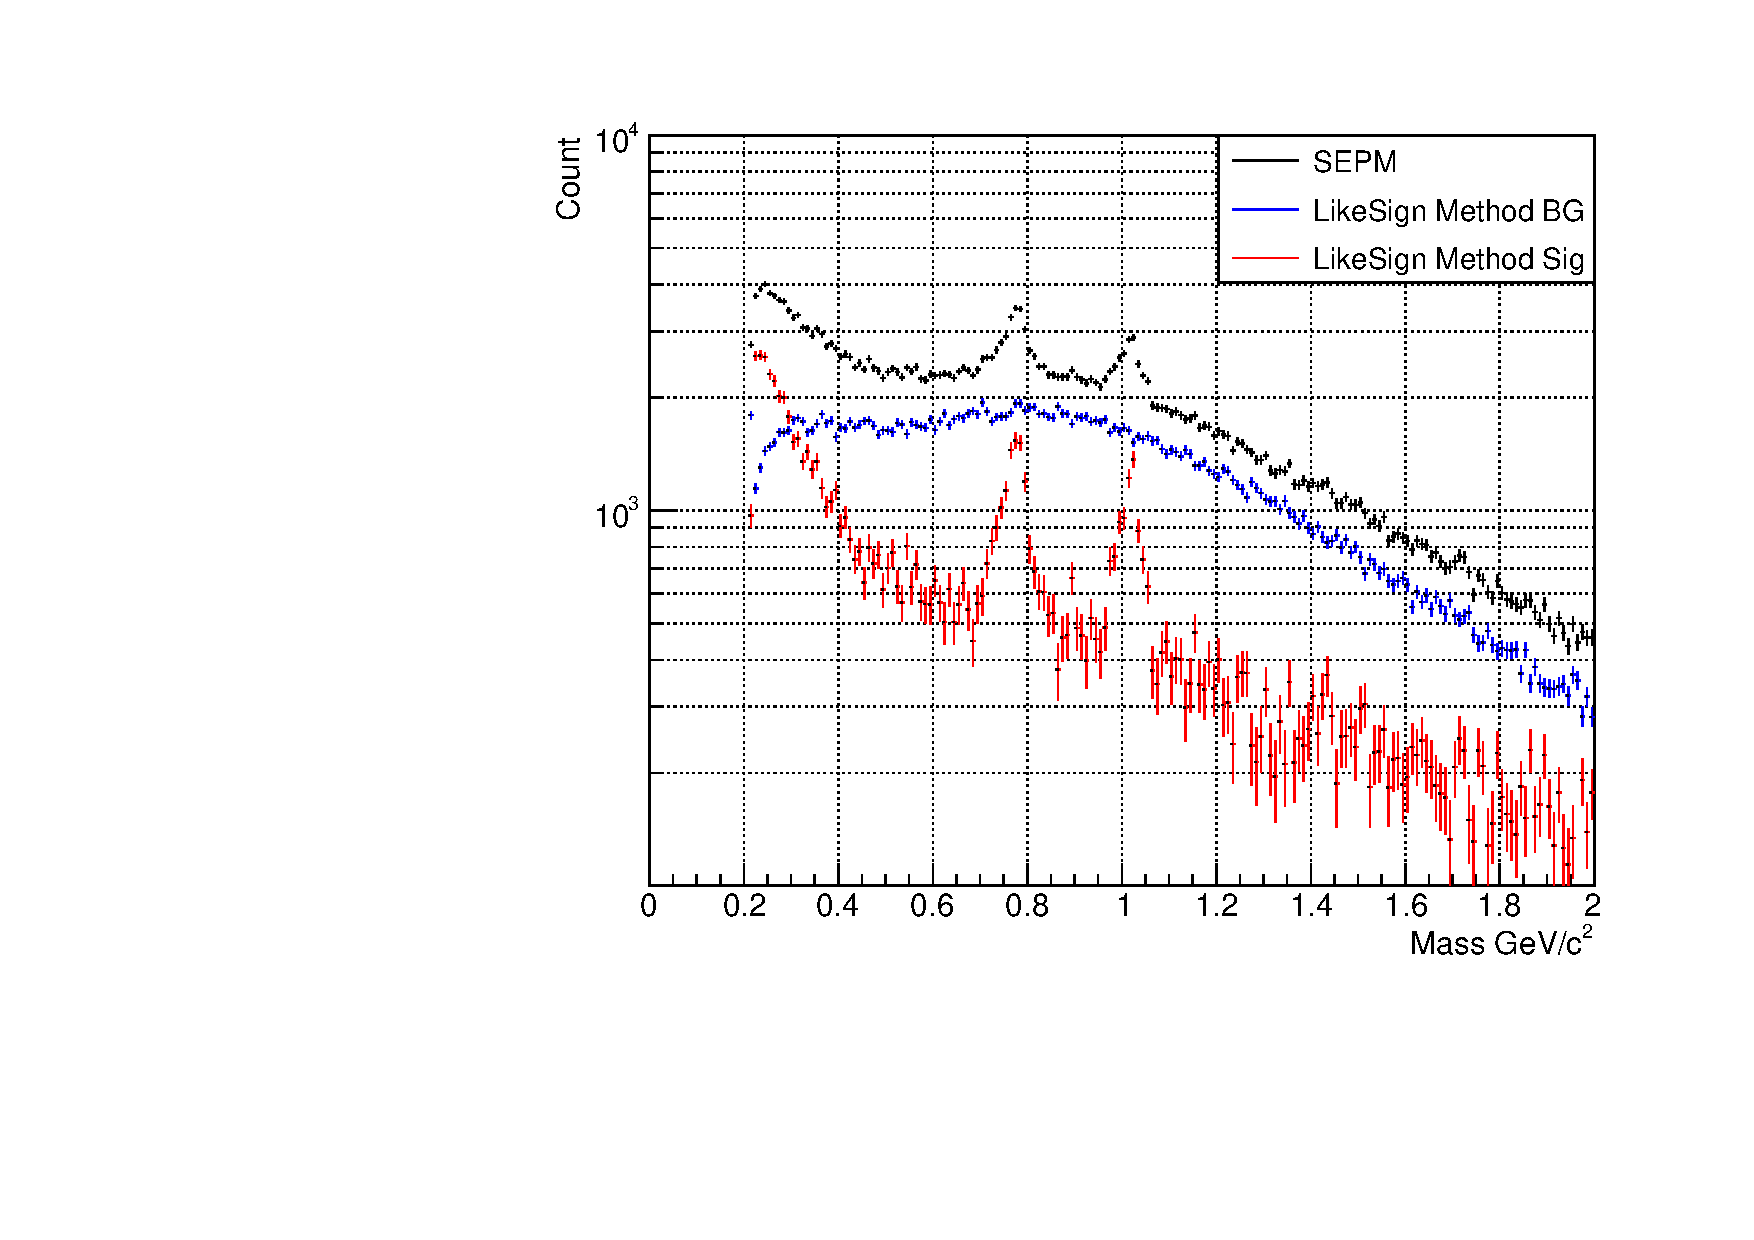
\includegraphics[width=\textwidth]{fig/3_4_4_chi2_20.pdf}
                    \captionsetup{labelformat=empty}
                    \caption{MFT-MCH matching $\chi^2 < 20$}
                    \label{fig:chi2_20}
                \end{minipage}
                \hfill
                \begin{minipage}{0.45\textwidth}
                    \centering
                    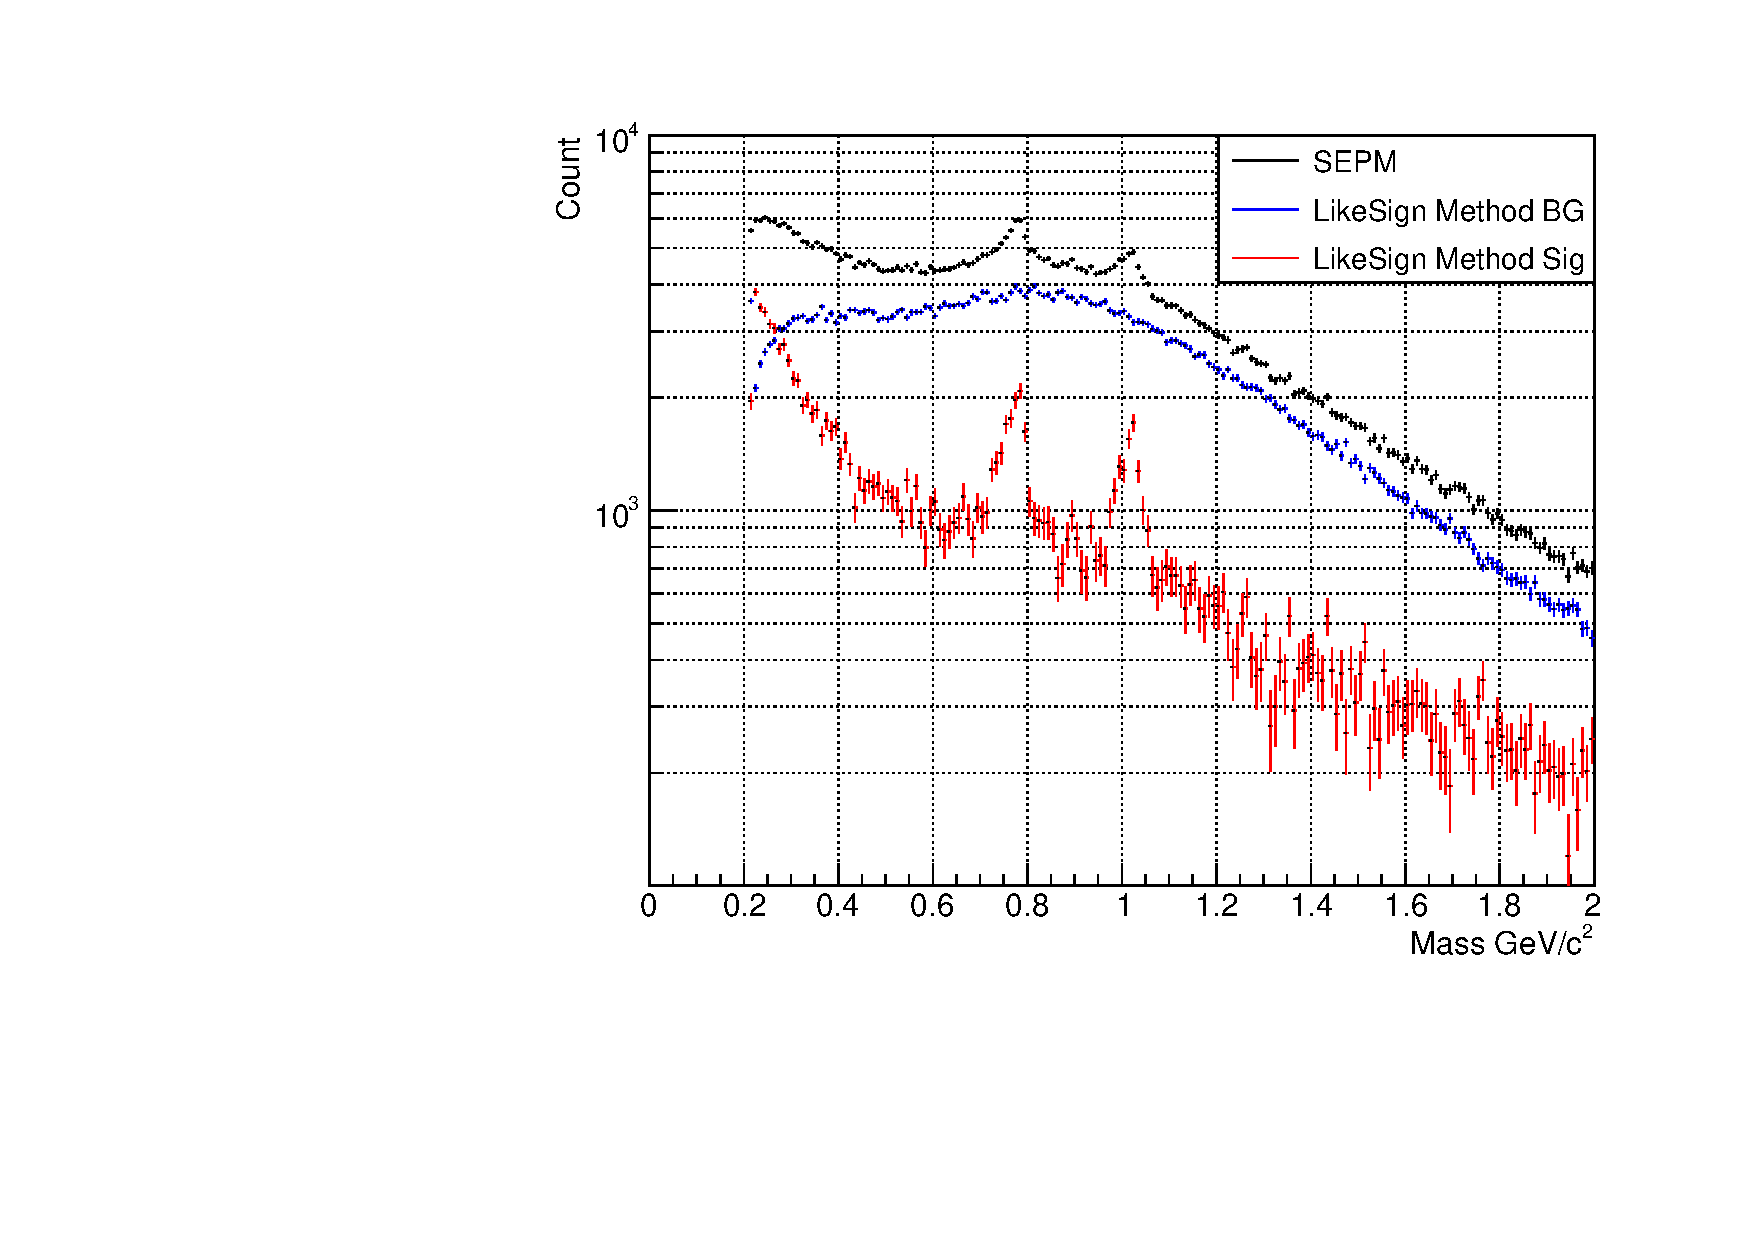
\includegraphics[width=\textwidth]{fig/3_4_4_chi2_40.pdf}
                    \captionsetup{labelformat=empty}
                    \caption{MFT-MCH matching $\chi^2 < 40$}
                    \label{fig:chi2_40}
                \end{minipage}
                \\
                \vspace{1em}
                \begin{minipage}{0.45\textwidth}
                    \centering
                    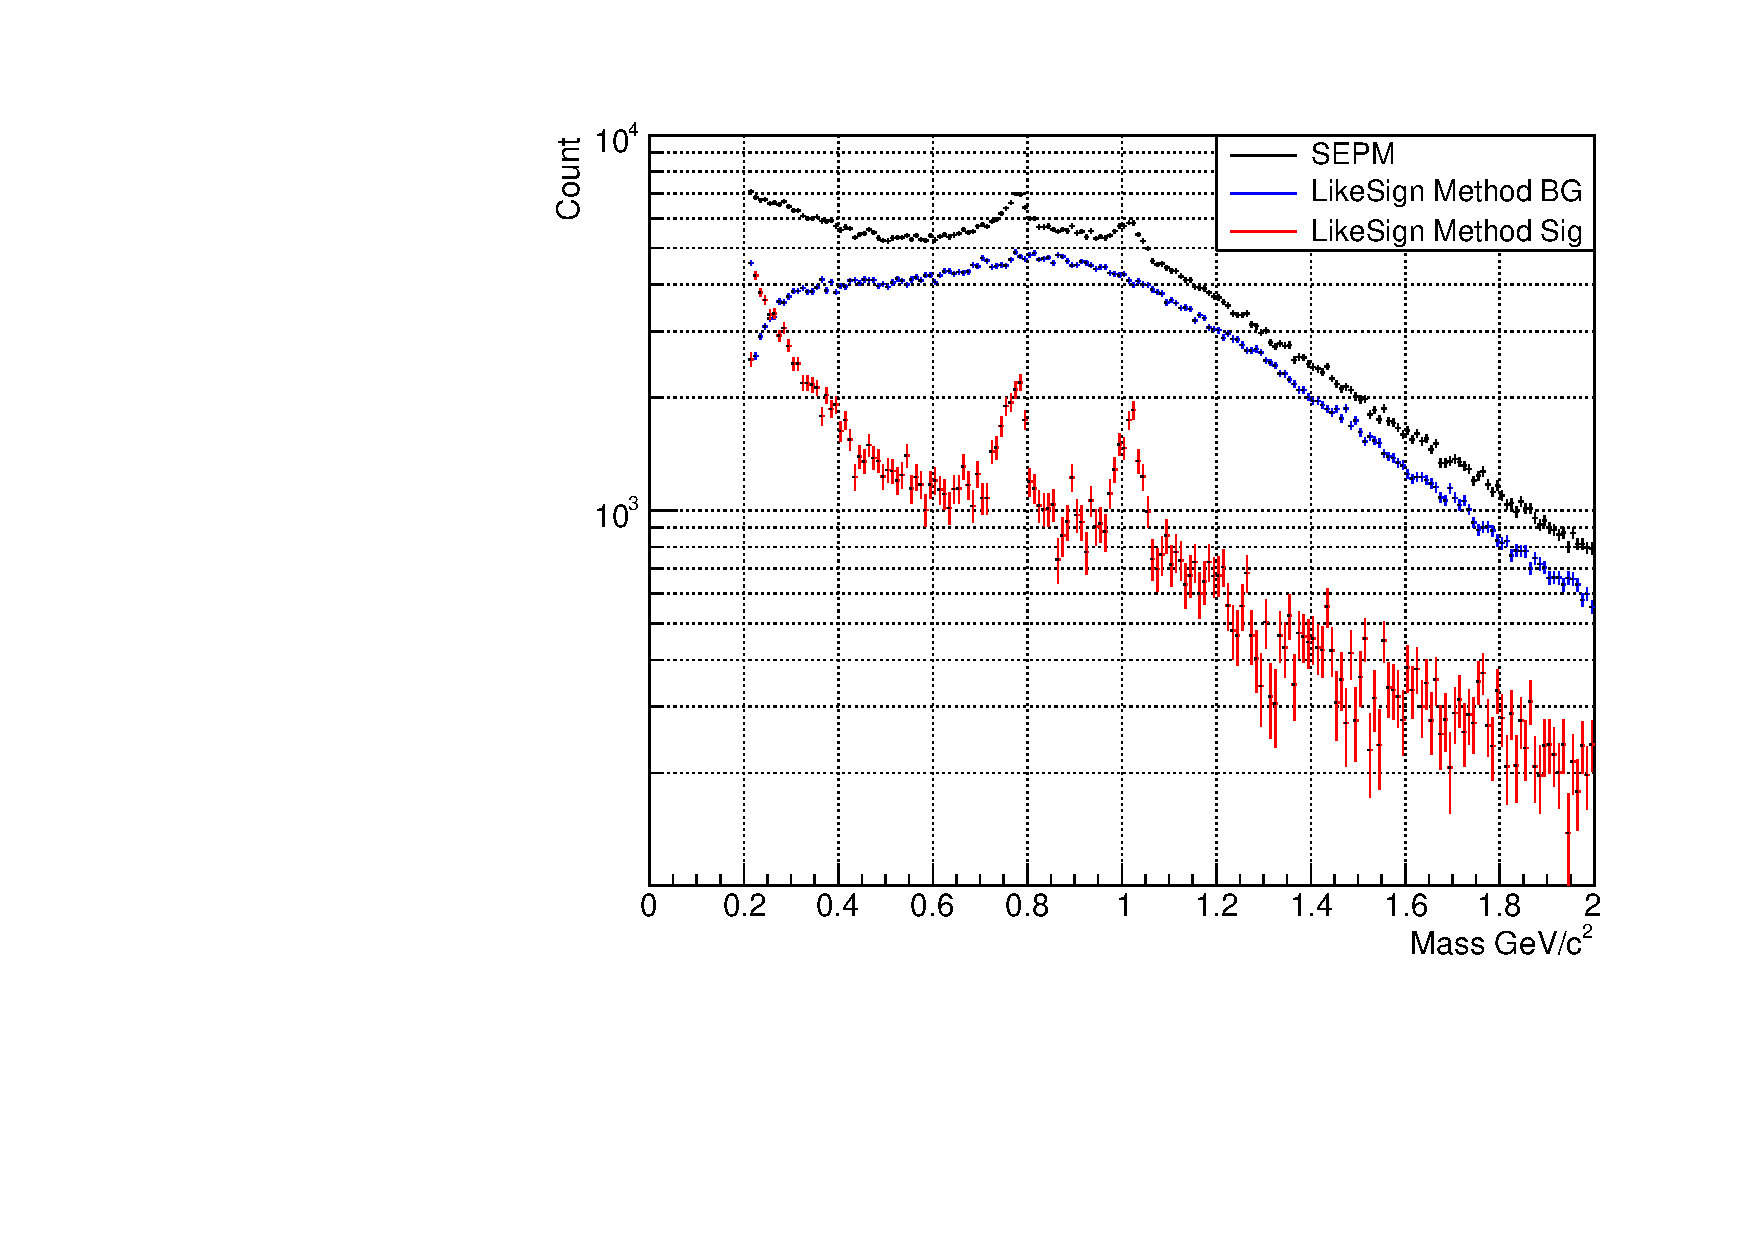
\includegraphics[width=\textwidth]{fig/3_4_4_chi2_60.pdf}
                    \captionsetup{labelformat=empty}
                    \caption{MFT-MCH matching $\chi^2 < 60$}
                    \label{fig:chi2_60}
                \end{minipage}
                \hfill
                \begin{minipage}{0.45\textwidth}
                    \centering
                    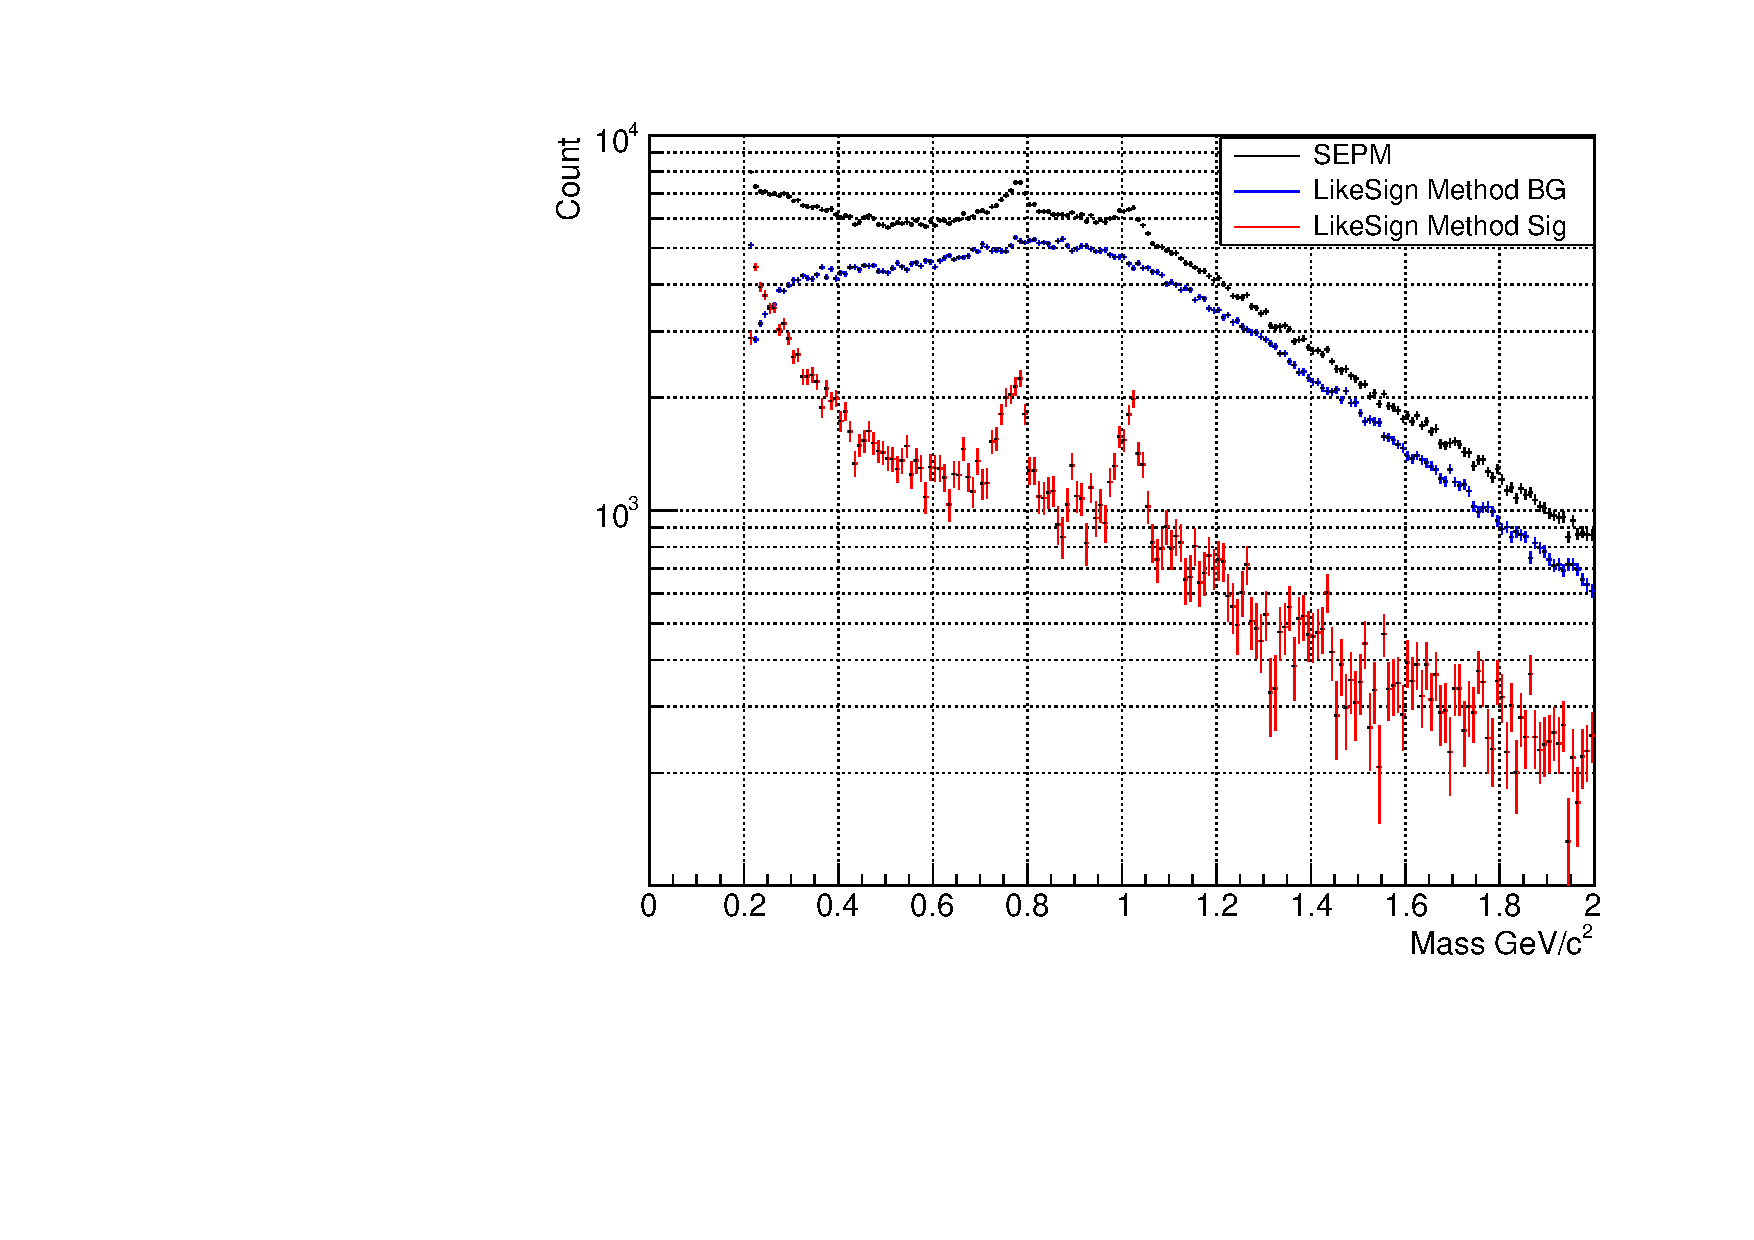
\includegraphics[width=\textwidth]{fig/3_4_4_chi2_80.pdf}
                    \captionsetup{labelformat=empty}
                    \caption{MFT-MCH matching $\chi^2 < 80$} 
                    \label{fig:chi2_80}
                \end{minipage}
                \\
                \vspace{1em}
                \begin{minipage}{0.45\textwidth}
                    \centering
                    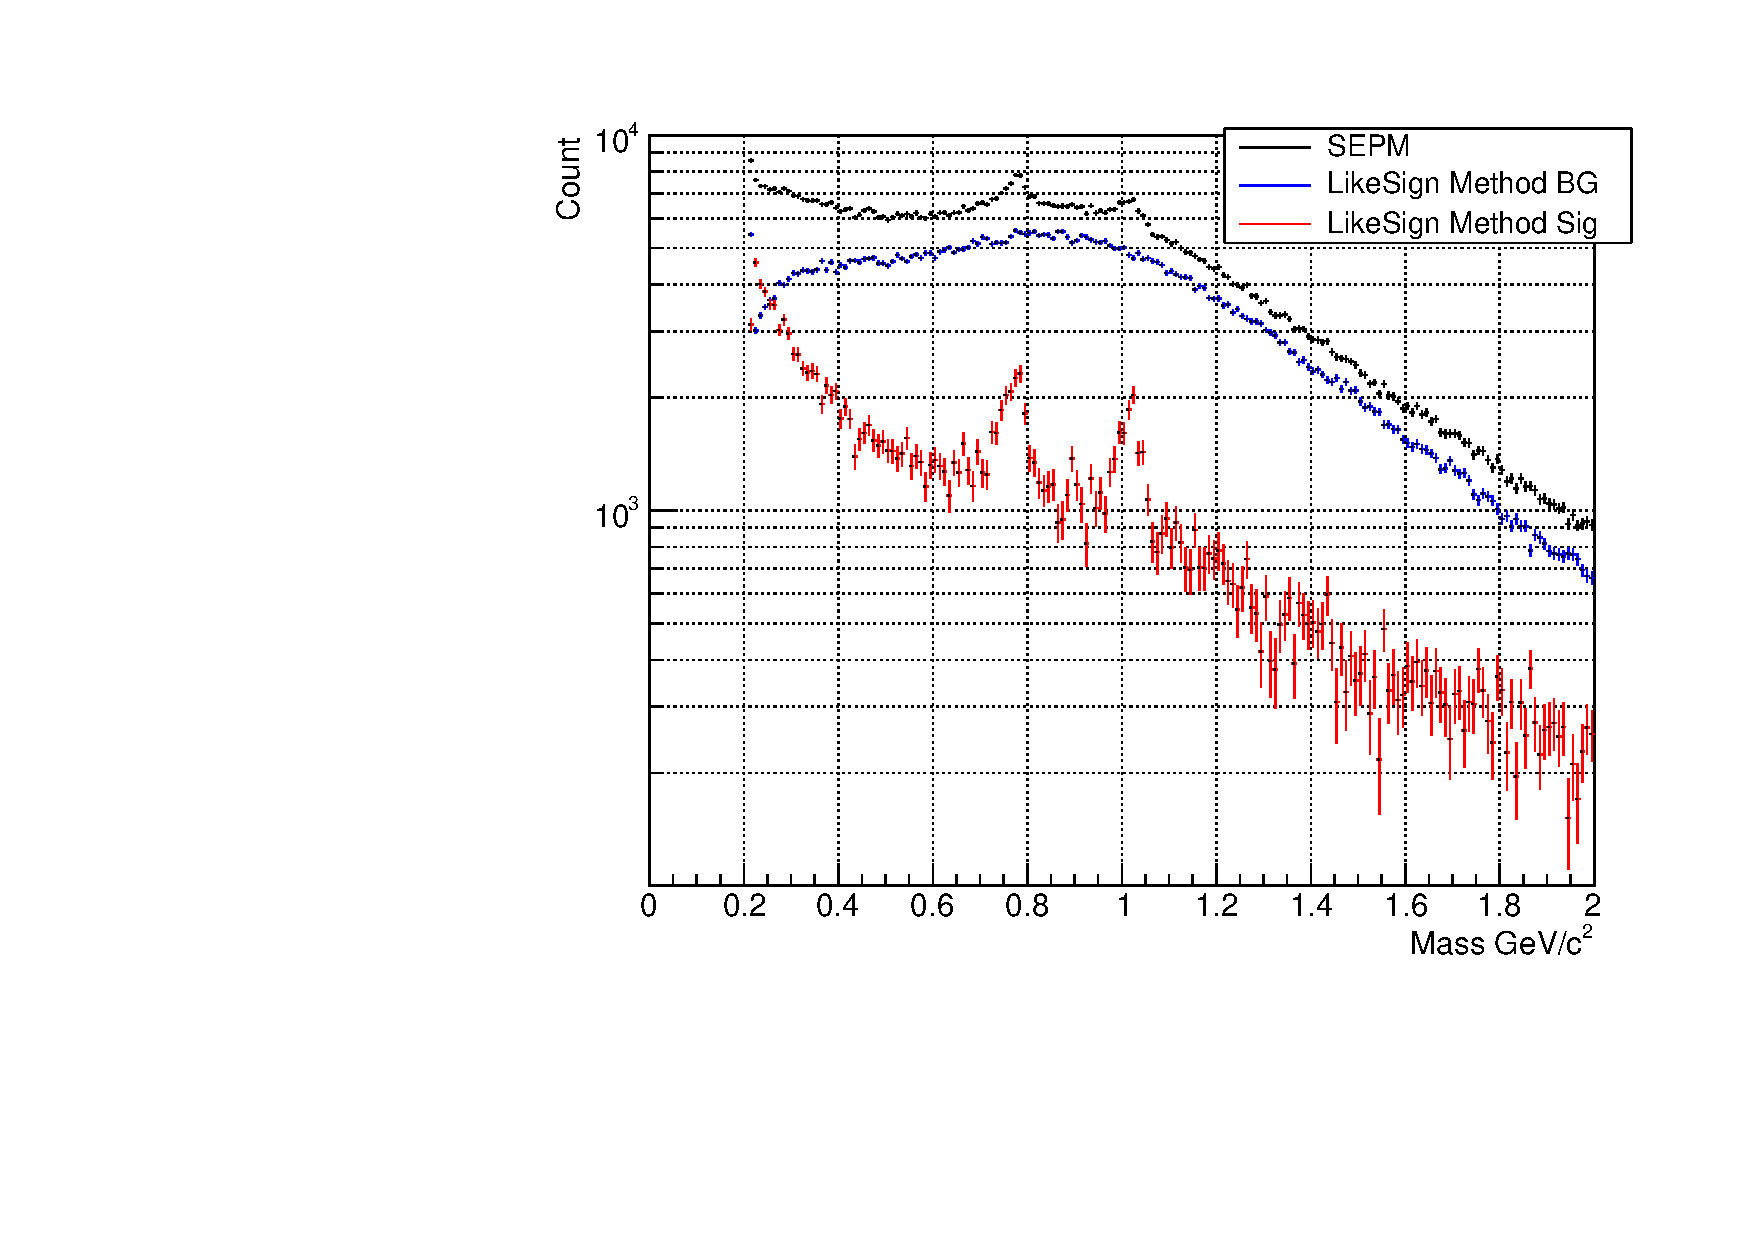
\includegraphics[width=\textwidth]{fig/3_4_4_chi2_100.pdf}
                    \captionsetup{labelformat=empty}
                    \caption{MFT-MCH matching $\chi^2 < 100$}
                    \label{fig:chi2_100}
                \end{minipage}
                \hfill
                \begin{minipage}{0.45\textwidth}
                    \centering
                    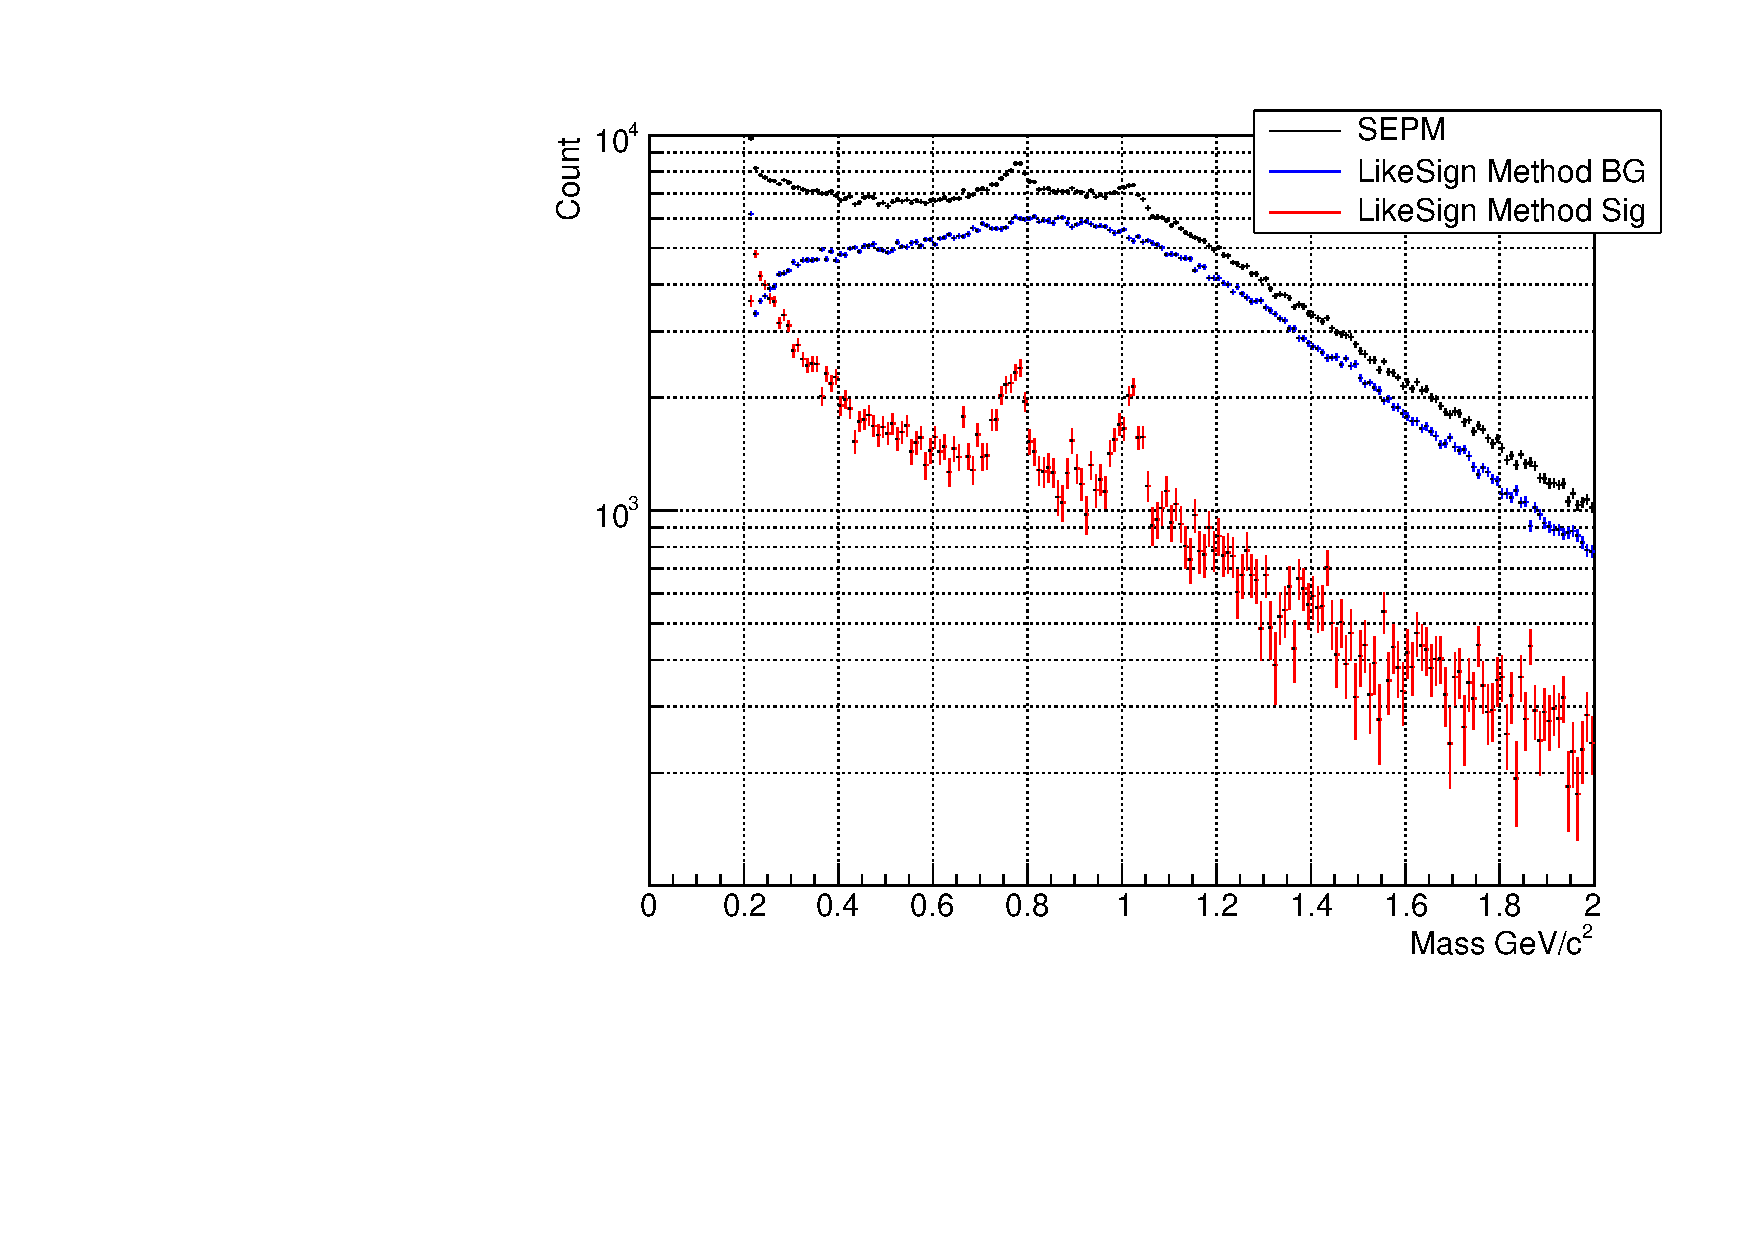
\includegraphics[width=\textwidth]{fig/3_4_4_chi2_200.pdf}
                    \captionsetup{labelformat=empty}
                    \caption{MFT-MCH matching $\chi^2 < 200$}
                    \label{fig:chi2_200}
                \end{minipage}
            \end{figure}
            Similarly, from the fit results, the yields for $\omega \rightarrow \mu\mu$ and $\phi \rightarrow \mu\mu$ were obtained. These yields were then normalized by dividing by the number of dimuons in the same mass region, and the optimization was performed to maximize $S/\sqrt{S+BG}$.\@ The resulting plot is shown below, where the x-axis is the matching $\chi^2$ and the y-axis is $S/\sqrt{S+BG}$.\@ From this, it is observed that the optimal value for the matching $\chi^2$ is $\chi^2 <$ 30.\@
            \begin{figure}[htbp]
                \centering
                % Left figure
                \begin{minipage}{0.45\textwidth} % minipage for width specification
                    \centering
                    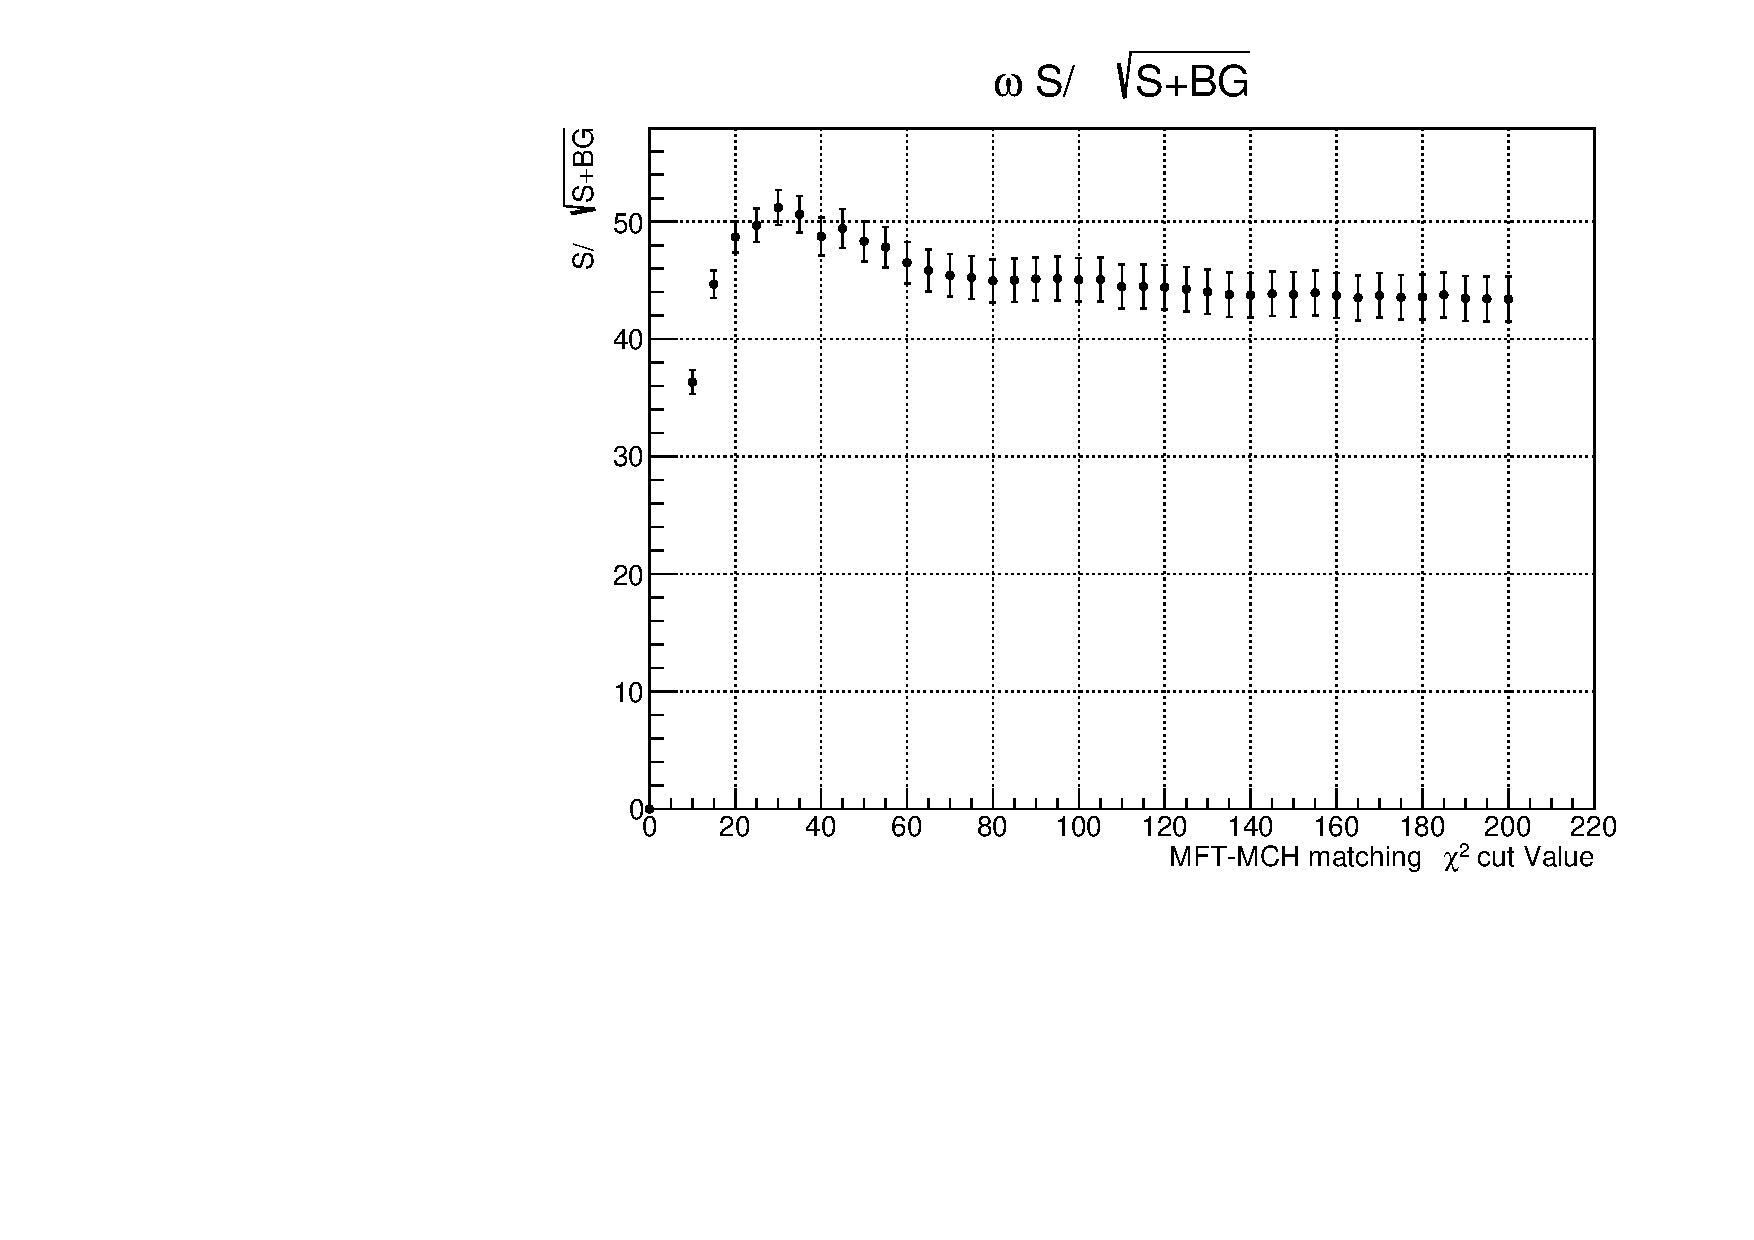
\includegraphics[width=\textwidth]{fig/3_4_4_omega_significance.pdf} % Left image
                    \caption{$\omega$ figure of merit}
                    \label{fig:omega_significance}
                \end{minipage}
                % Right figure
                \hfill
                \begin{minipage}{0.45\textwidth}
                    \centering
                    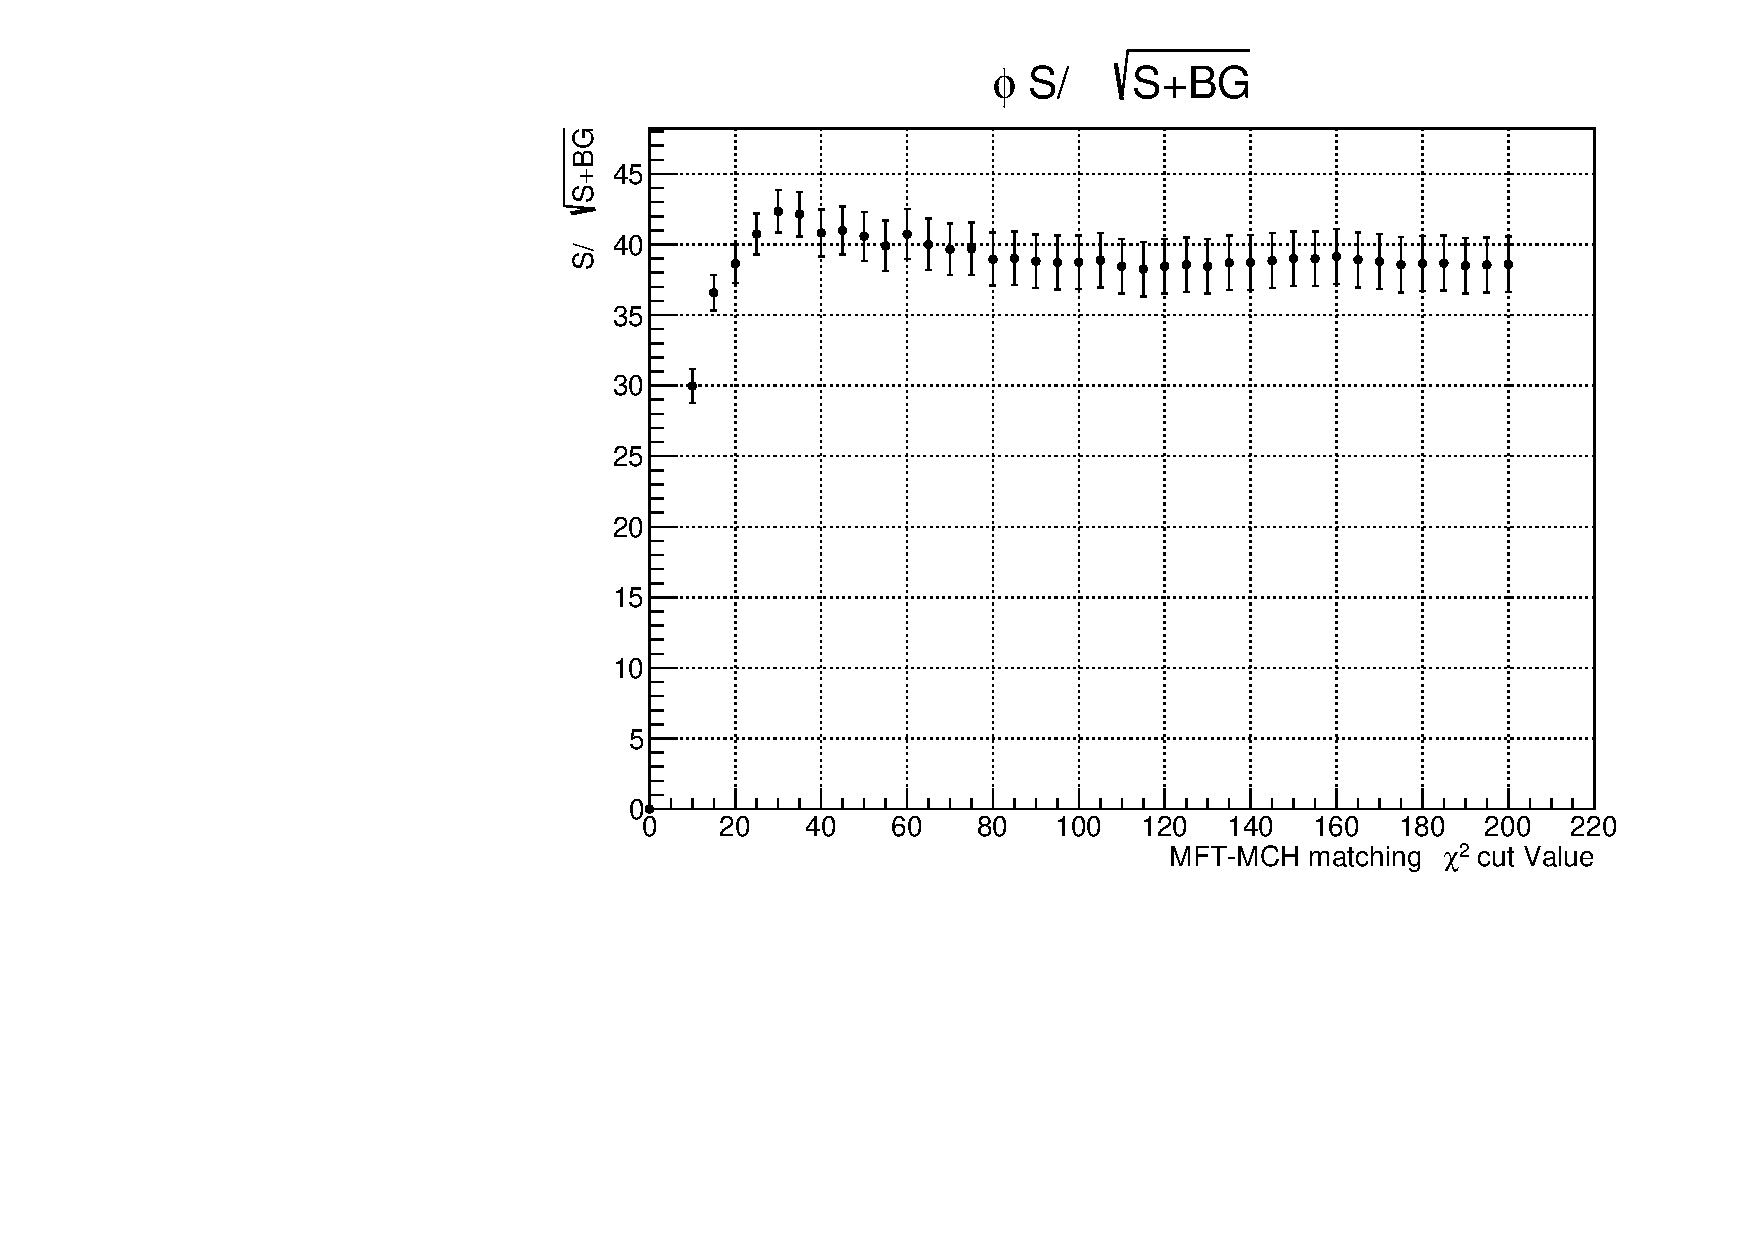
\includegraphics[width=\textwidth]{fig/3_4_4_phi_significance.pdf} % Right image
                    \caption{$\phi$ figure of merit}
                    \label{fig:phi_significance}
                \end{minipage}
            \end{figure}
            \subsection{Fake Match Track Removal Analysis of MFT-MCH-MID Track using MFT Track $\eta$ - MCH Track $\eta$}
            \label{Analysis:Matching}
                The matching of MFT Tracks located before the hadron absorption pair and MCH Tracks located behind them is important for the quality of physical quantities such as single muon $p_T$ and $\eta$. Here, we performed an analysis to remove MFT-MCH-MID tracks, which match incorrect tracks, by applying cuts to the already reconstructed Global Tracks using three detectors. The dataset used is LHC24b1, which is a Monte Carlo dataset for $pp\sqrt{s}=13.6$TeV minimum-bias events. This simulation data is detailed in % \ref{Appendix:compair_Real_and_MC}.
                
                The tracks reconstructed with MFT-MCH-MID tracks, as shown in \ref{Analysis:Matching:eta}, include tracks reconstructed outside the acceptance. The black histogram shows the $\eta$ distribution of the reconstructed Global Tracks. Blue represents the $\eta$ distribution of fake match tracks, and red represents the $\eta$ distribution of correct match tracks. The green distribution corresponds to the true $\eta$ distribution for the black tracks. By comparing the green and black distributions, we observe that muons outside the acceptance are reconstructed, and they form the distribution of fake matches. 
                To remove such tracks, we applied the following $\Delta \eta$ cut:
                \begin{eqnarray}
                    \Delta \eta = \text{MFT} \, \eta - \text{MCH} \, \eta  
                \end{eqnarray}
                We calculated $\Delta \eta$ for each track and examined the distributions of fake match tracks and correct match tracks. The resulting distributions are shown in the following figure, where blue represents the fake match distribution and red represents the correct match distribution.
                \begin{figure}[htbp]
                    \centering
                    % Left figure
                    \begin{minipage}{0.45\textwidth} % Specify width with minipage
                        \centering
                        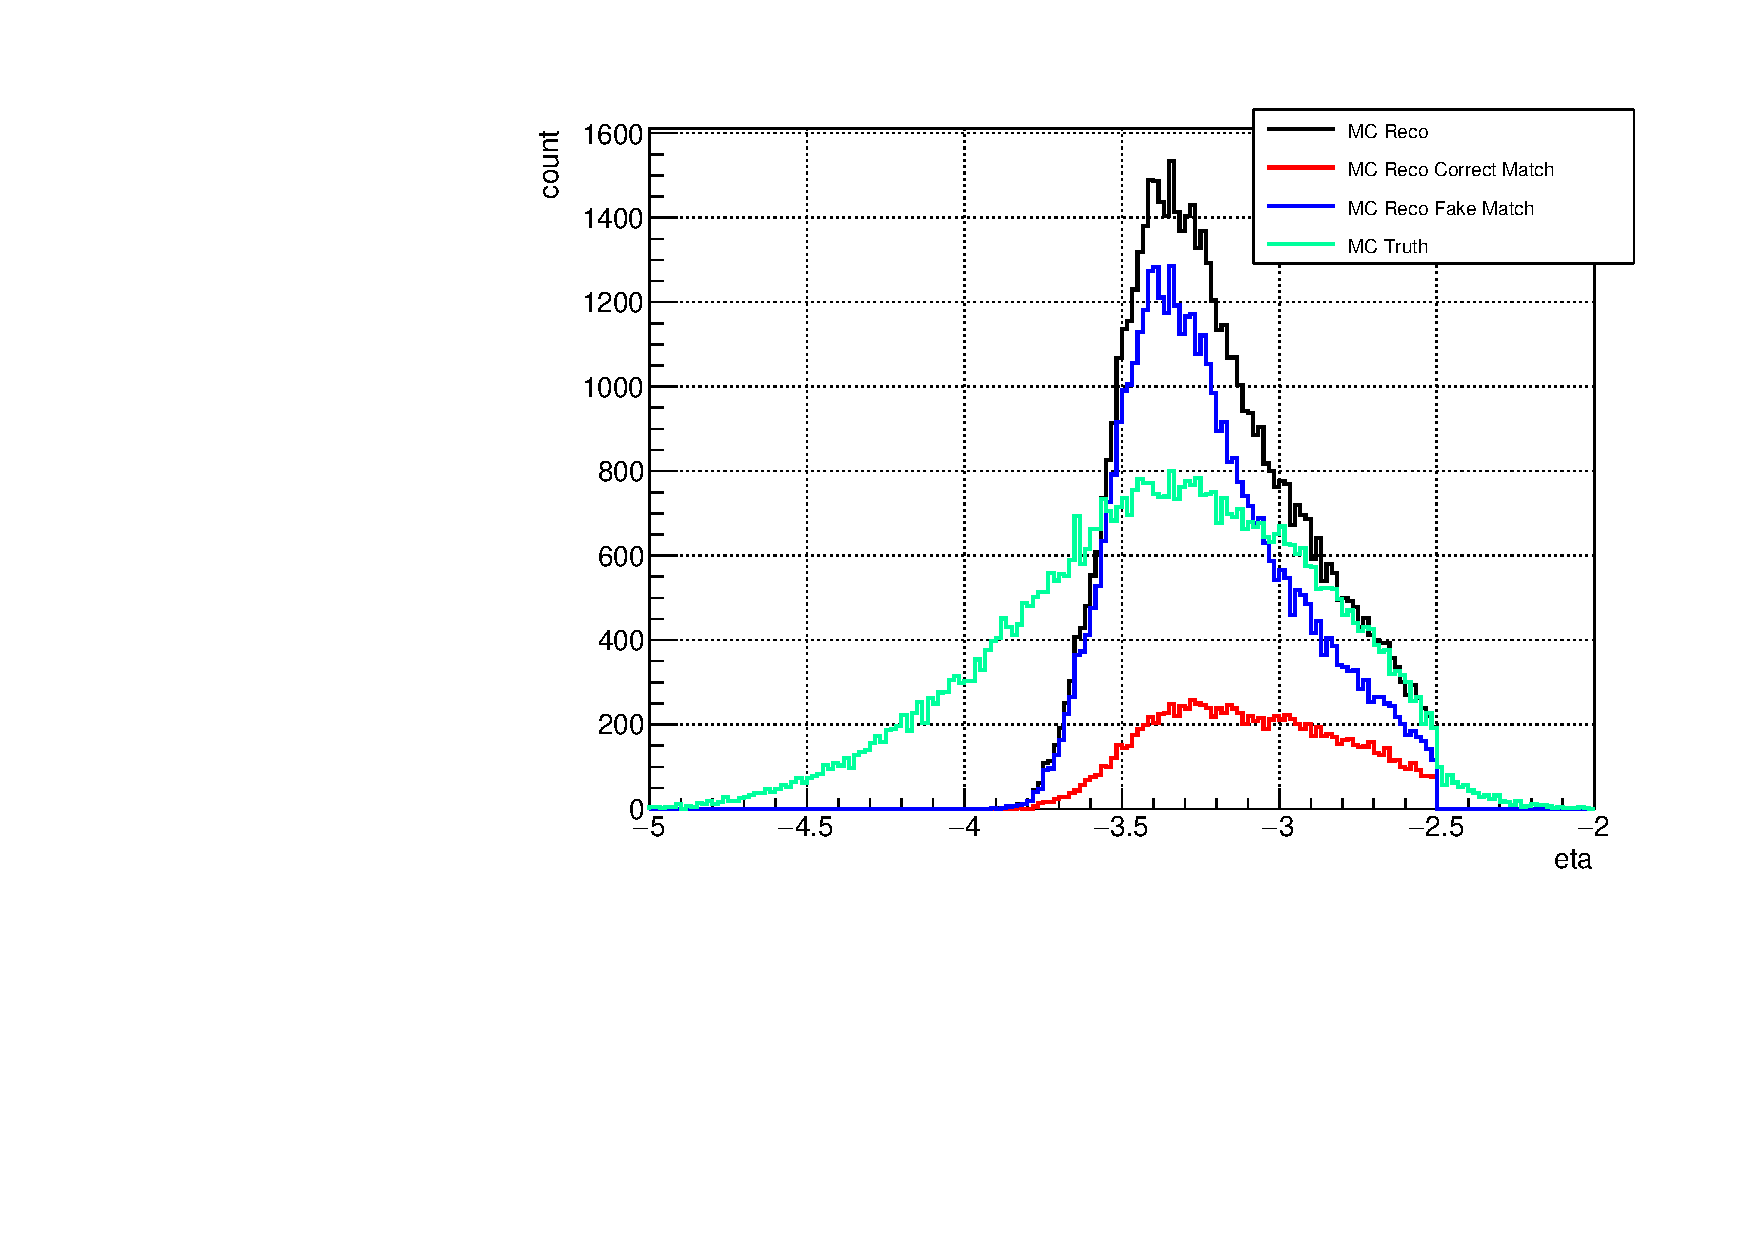
\includegraphics[width=\textwidth]{fig/3_3_matching_eta_comp.pdf} % Left image
                        \caption{MFT-MCH-MID Track $\eta$}
                        \label{Analysis:Matching:eta}
                    \end{minipage}
                    % Right figure
                    \hfill
                    \begin{minipage}{0.45\textwidth}
                        \centering
                        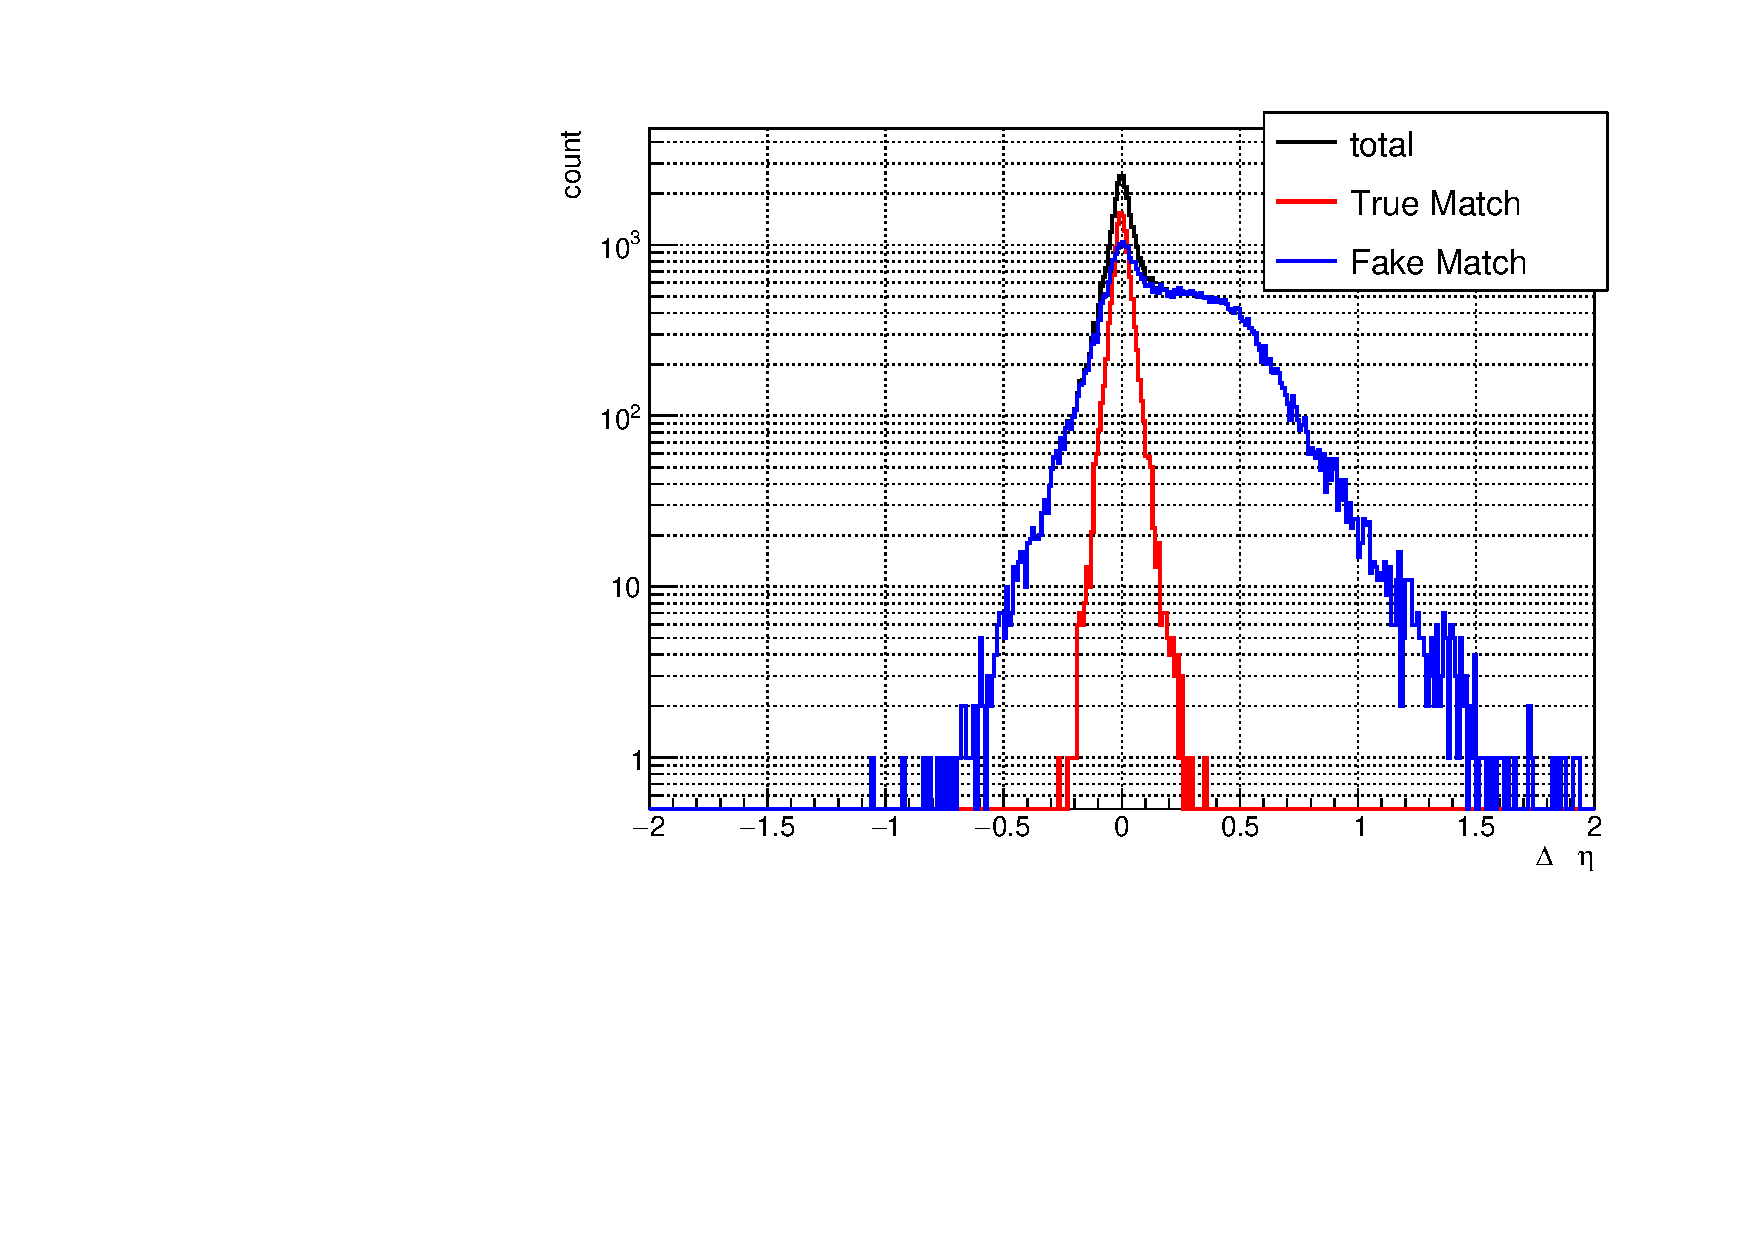
\includegraphics[width=\textwidth]{fig/3_3_DeltaEta_pt_0to30.pdf} % Right image
                        \caption{}
                        \label{Analysis:Matching:DeltaEta}
                    \end{minipage}
                \end{figure}
                From \ref{Analysis:Matching:DeltaEta}, we see that for $\Delta \eta > 0.2$, fake match tracks dominate. 
                To remove fake matches while preserving as many correct matches as possible, we applied a $\Delta \eta < 0.2$ cut. The distributions of each physical quantity after this cut are as follows.
                \begin{figure}[htbp]
                    \centering
                    % Left figure
                    \begin{minipage}{0.45\textwidth} % Specify width with minipage
                        \centering
                        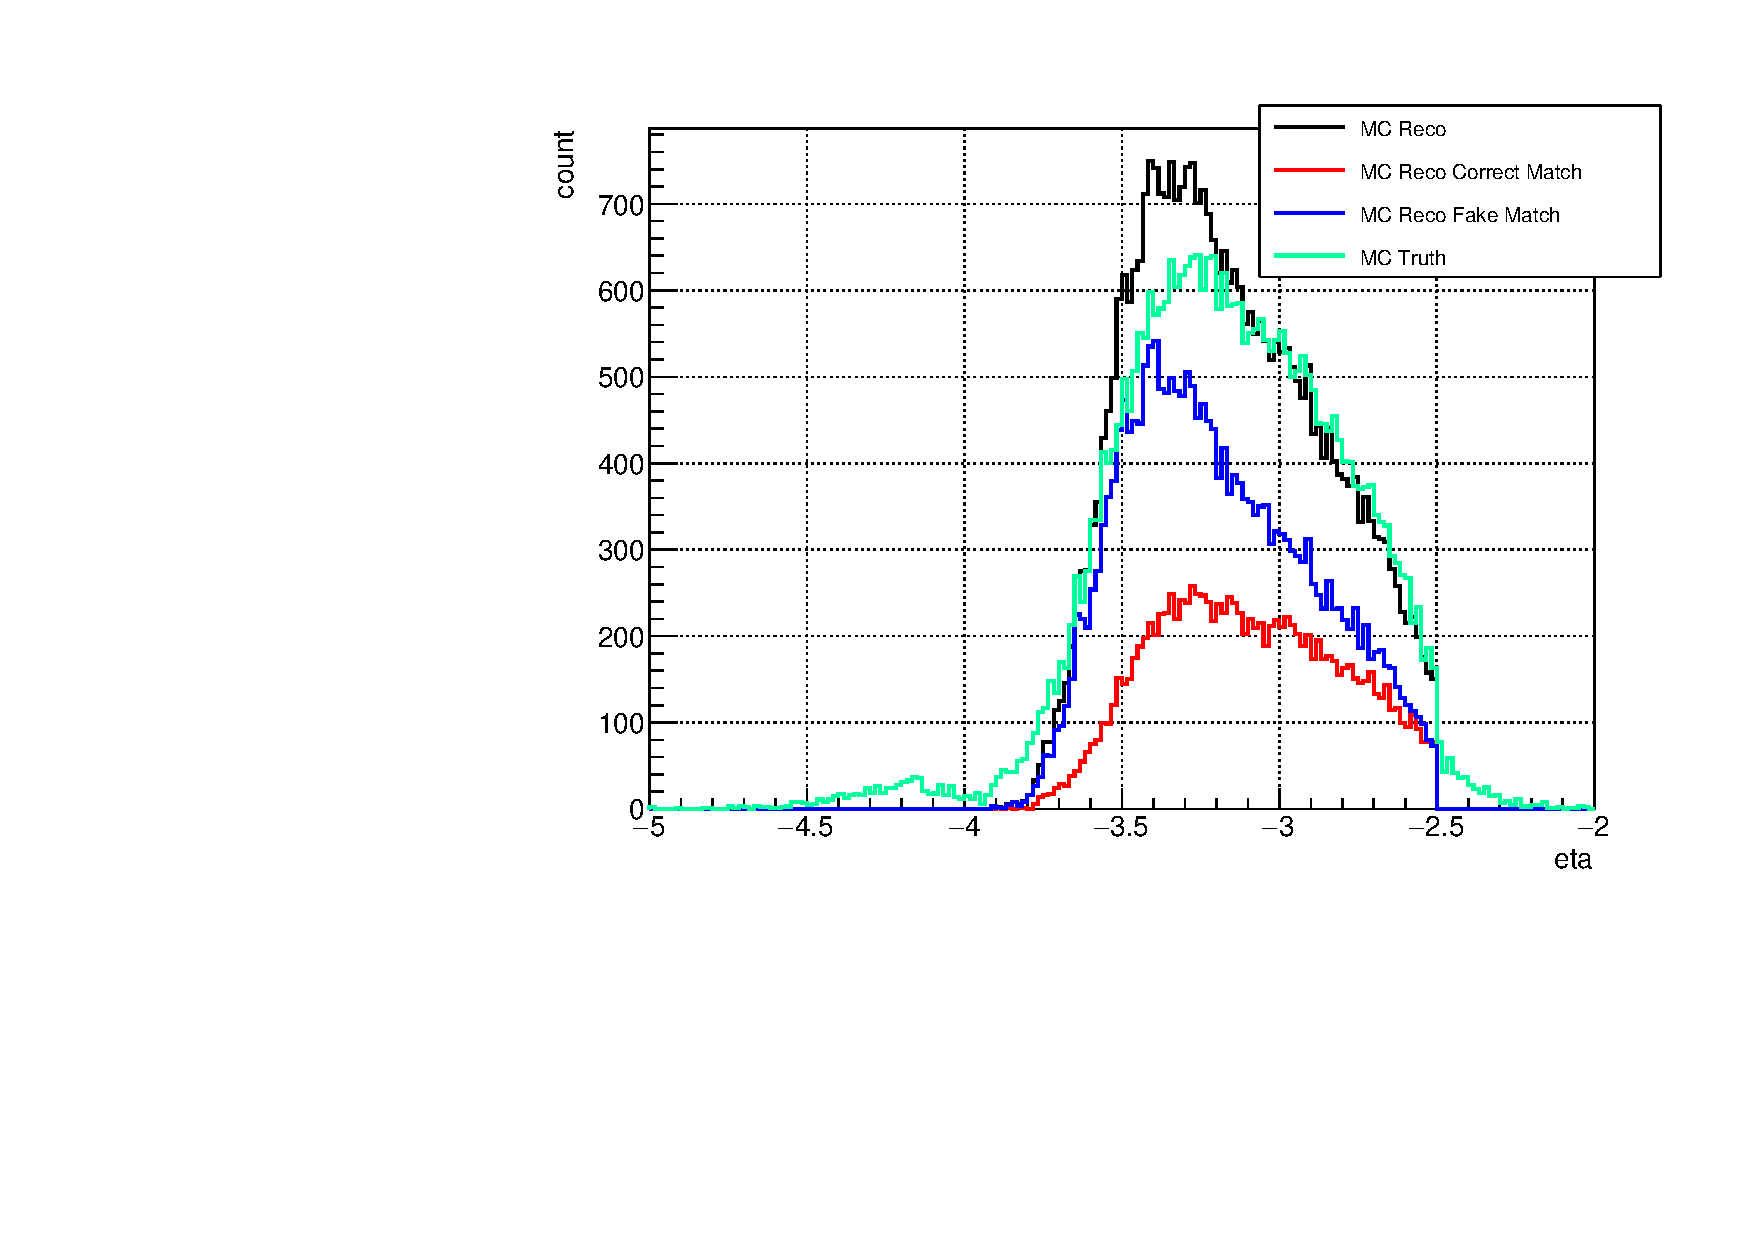
\includegraphics[width=\textwidth]{fig/3_3_eta_deltaetacut.pdf} % Left image
                        \caption{MFT-MCH-MID Track cutted $\eta$}
                        \label{Analysis:Matching:eta cutted}
                    \end{minipage}
                    % Right figure
                    \hfill
                    \begin{minipage}{0.45\textwidth}
                        \centering
                        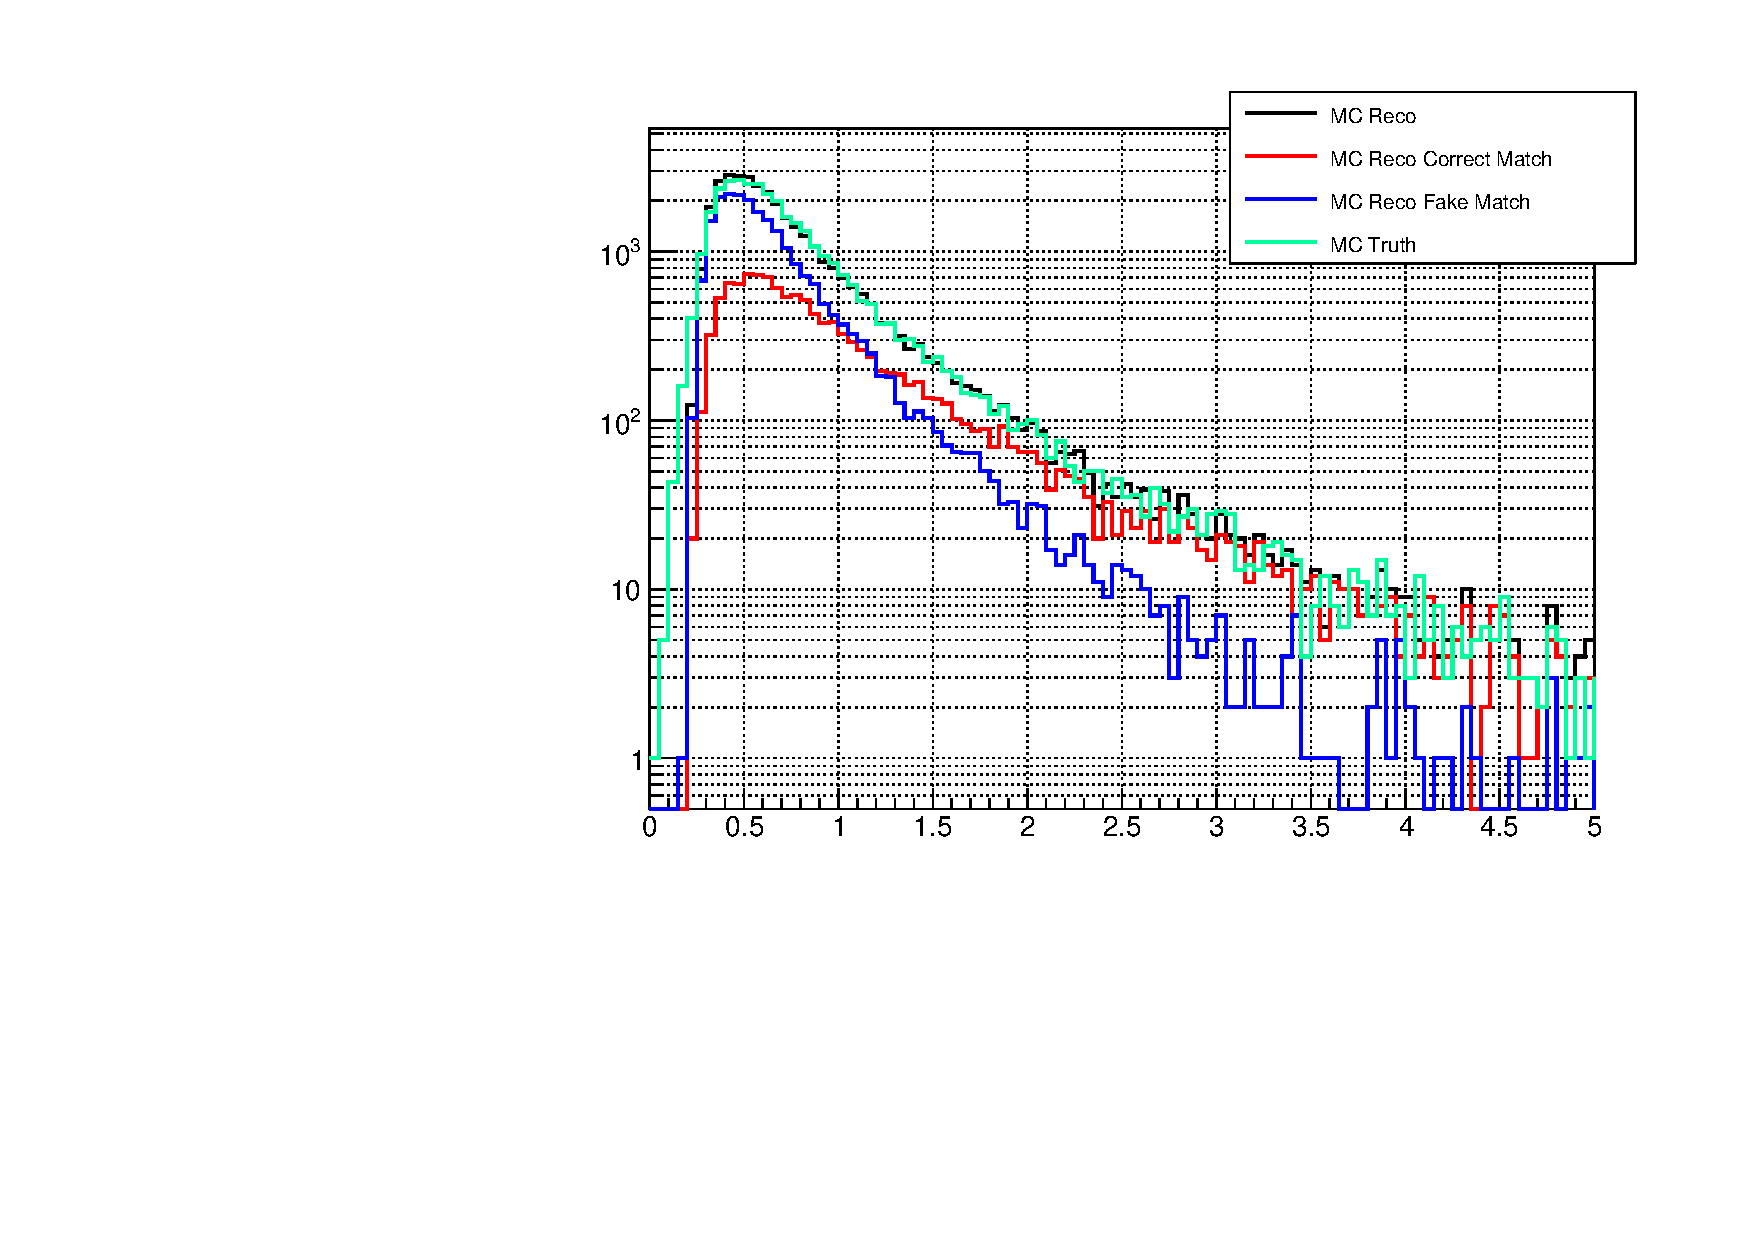
\includegraphics[width=\textwidth]{fig/3_3_pt_deltaetacut.pdf} % Right image
                        \caption{MFT-MCH-MID Track cutted $p_T$}
                        \label{Analysis:Matching:pt cutted}
                    \end{minipage}
                \end{figure}
                In \ref{Analysis:Matching:eta cutted}, all reconstructed tracks are shown in black, with red representing correct match tracks, blue representing fake match tracks, and green representing the true muon track distribution. By comparing the green distribution in \ref{Analysis:Matching:eta}, we observe that after the cut, tracks outside the acceptance have been removed. However, fake match tracks inside the acceptance remain. As shown in the $p_T$ distribution, there are still many fake match tracks at low $p_T$.\@
                The resolution of each physical quantity is shown below.
                \begin{figure}[htbp]
                    \centering
                    % Left figure
                    \begin{minipage}{0.3\textwidth} % Specify width with minipage
                        \centering
                        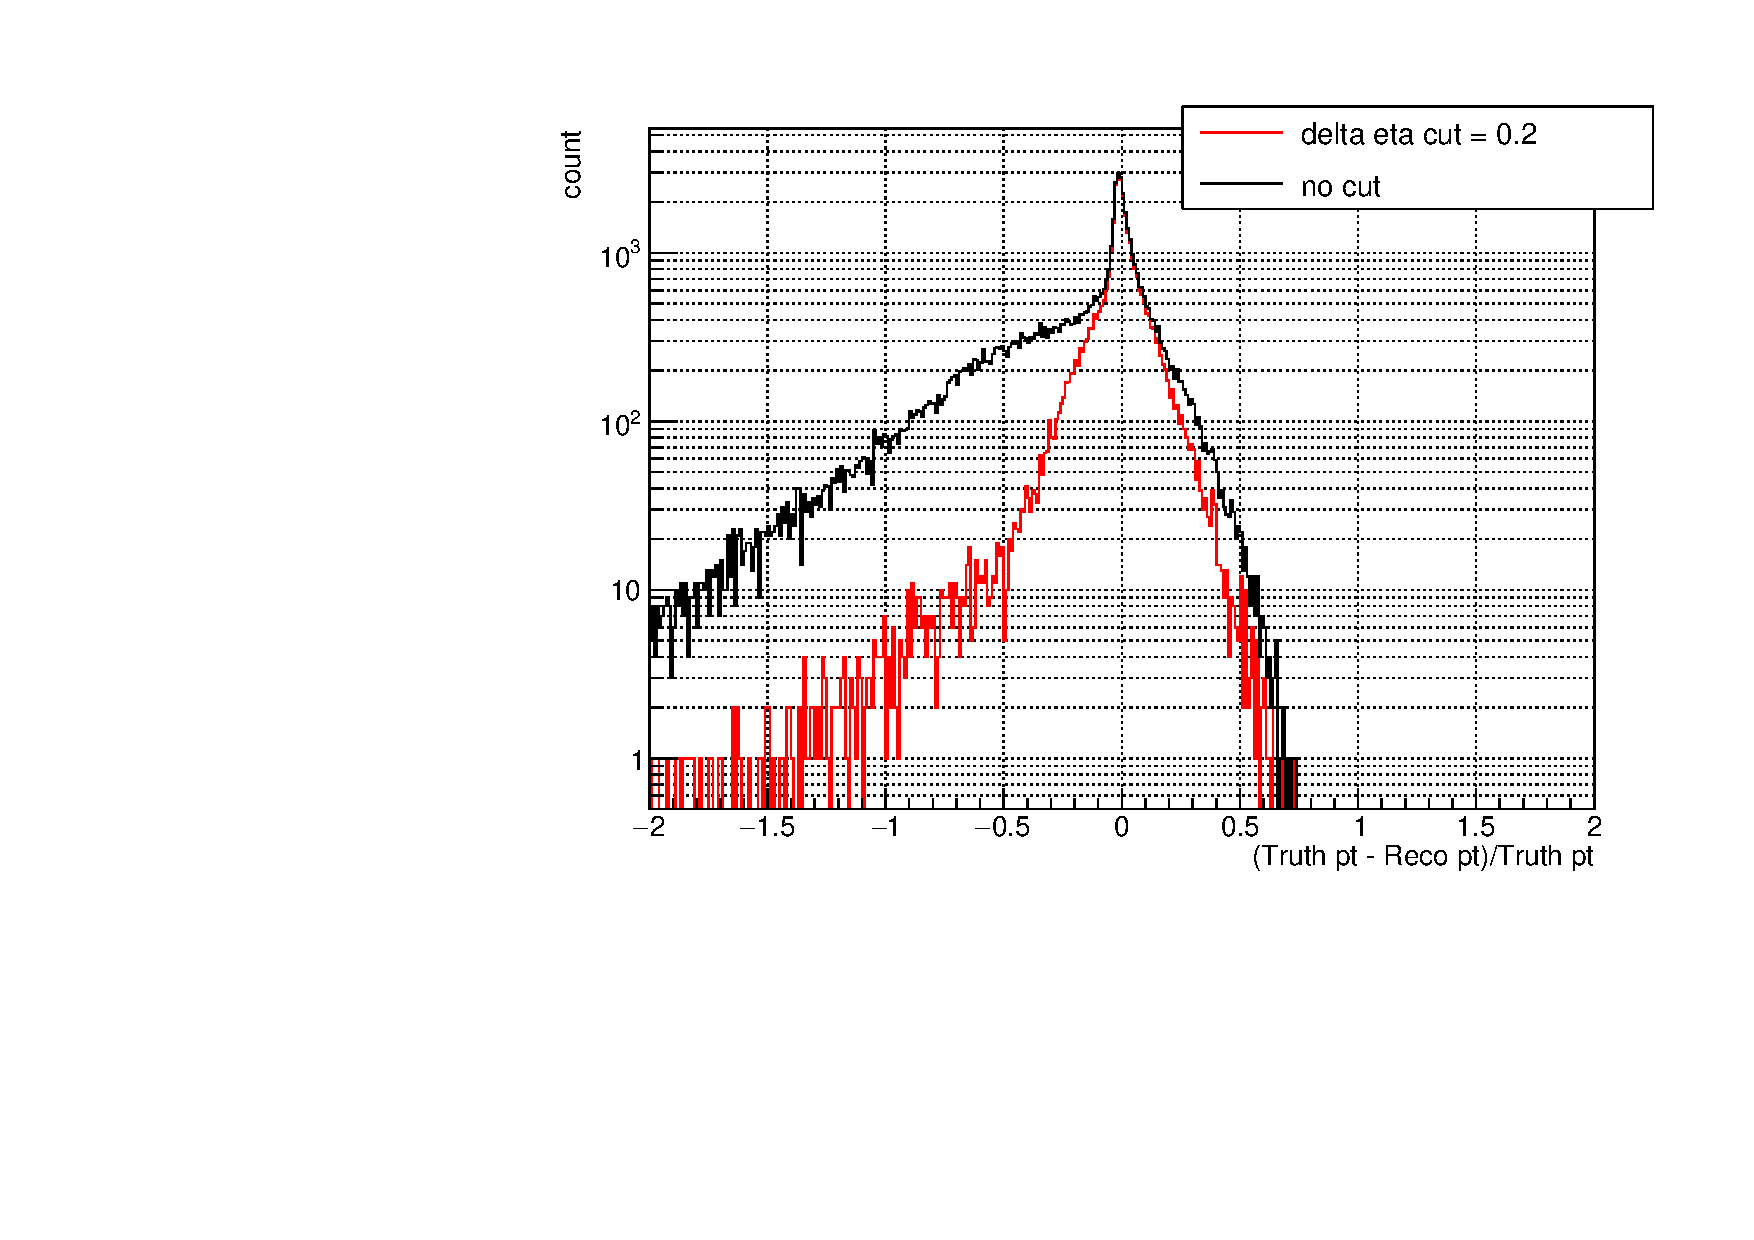
\includegraphics[width=\textwidth]{fig/3_3_pt_resolution.pdf} % Left image
                        \caption{MFT-MCH-MID Track cutted $\eta$}
                        \label{Analysis:Matching:pt resolution}
                    \end{minipage}
                    % Right figure
                    \begin{minipage}{0.3\textwidth}
                        \centering
                        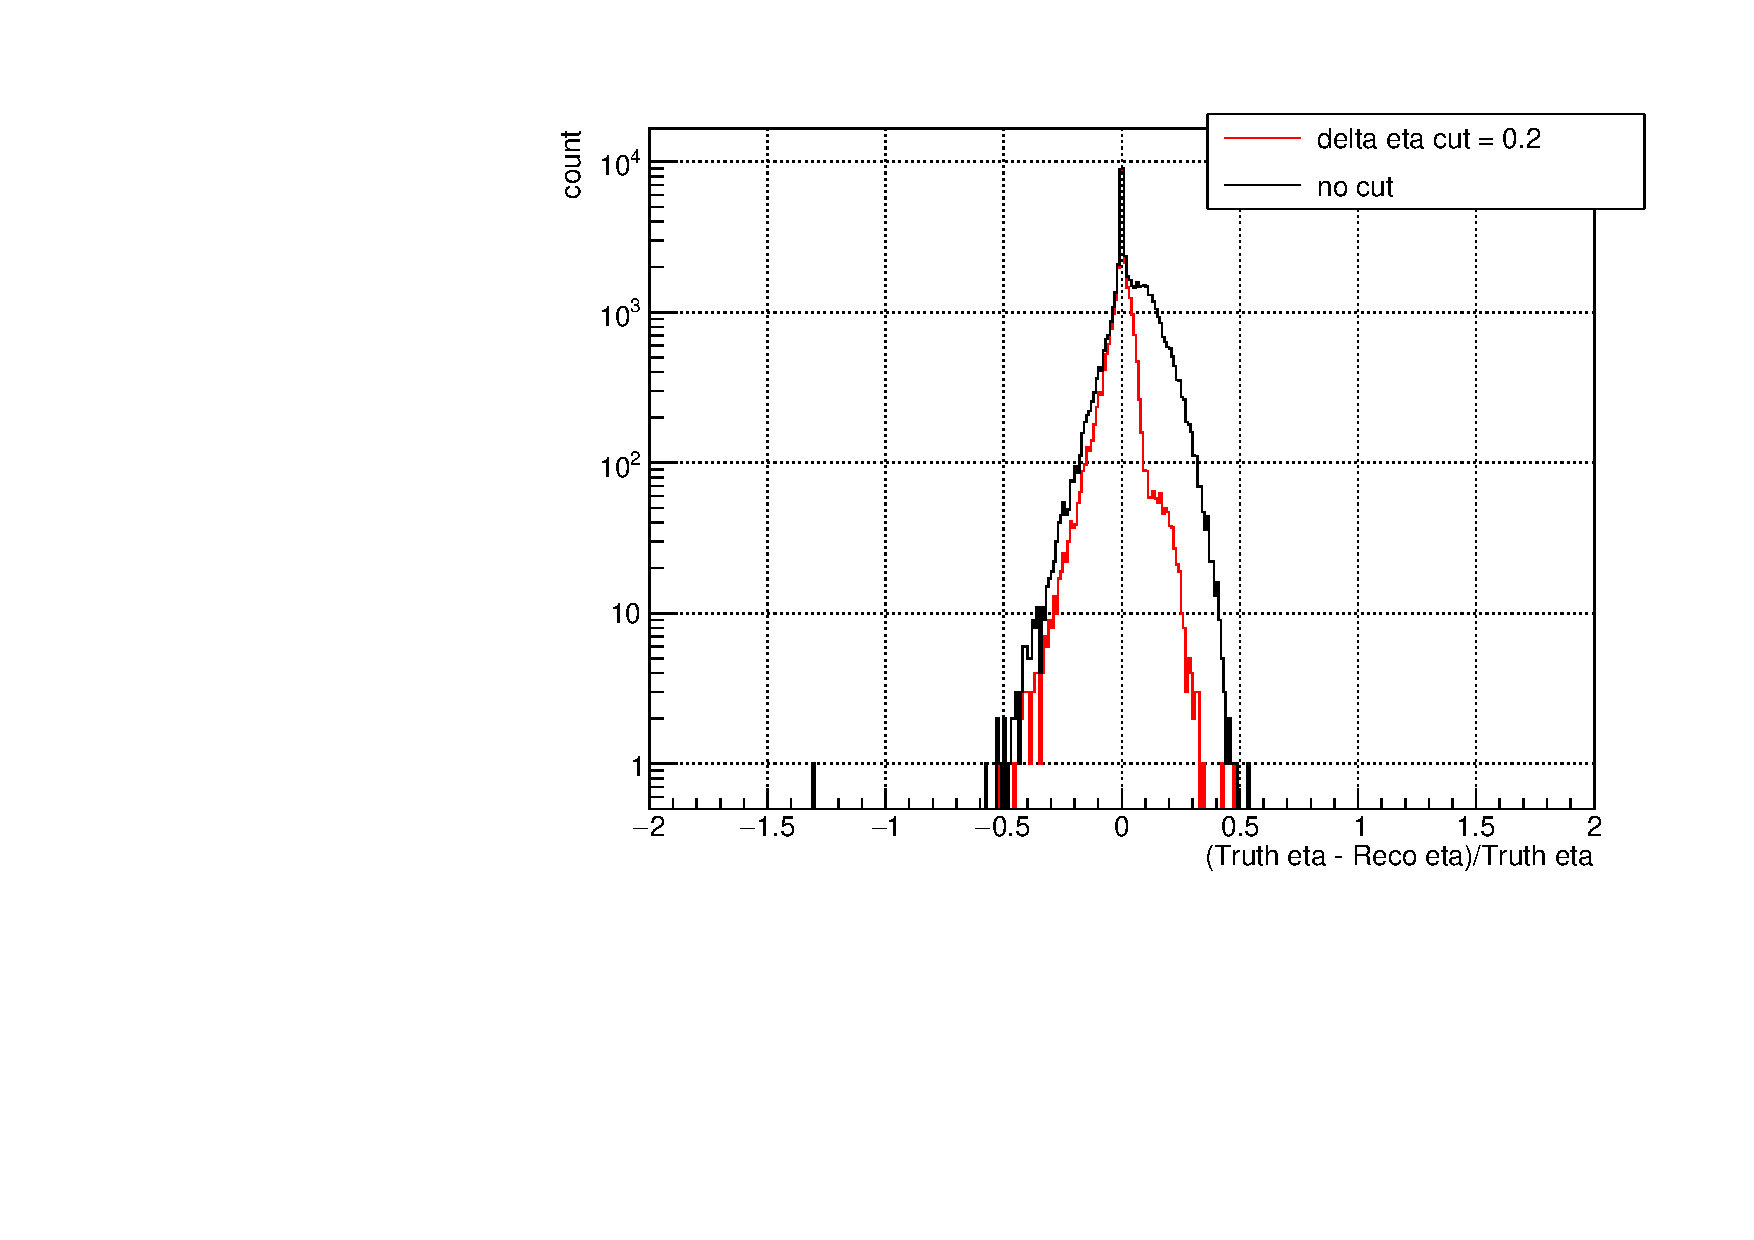
\includegraphics[width=\textwidth]{fig/3_3_eta_resolution.pdf} % Right image
                        \caption{MFT-MCH-MID Track cutted $p_T$}
                        \label{Analysis:Matching:eta resolution}
                    \end{minipage}
                    \begin{minipage}{0.3\textwidth}
                        \centering
                        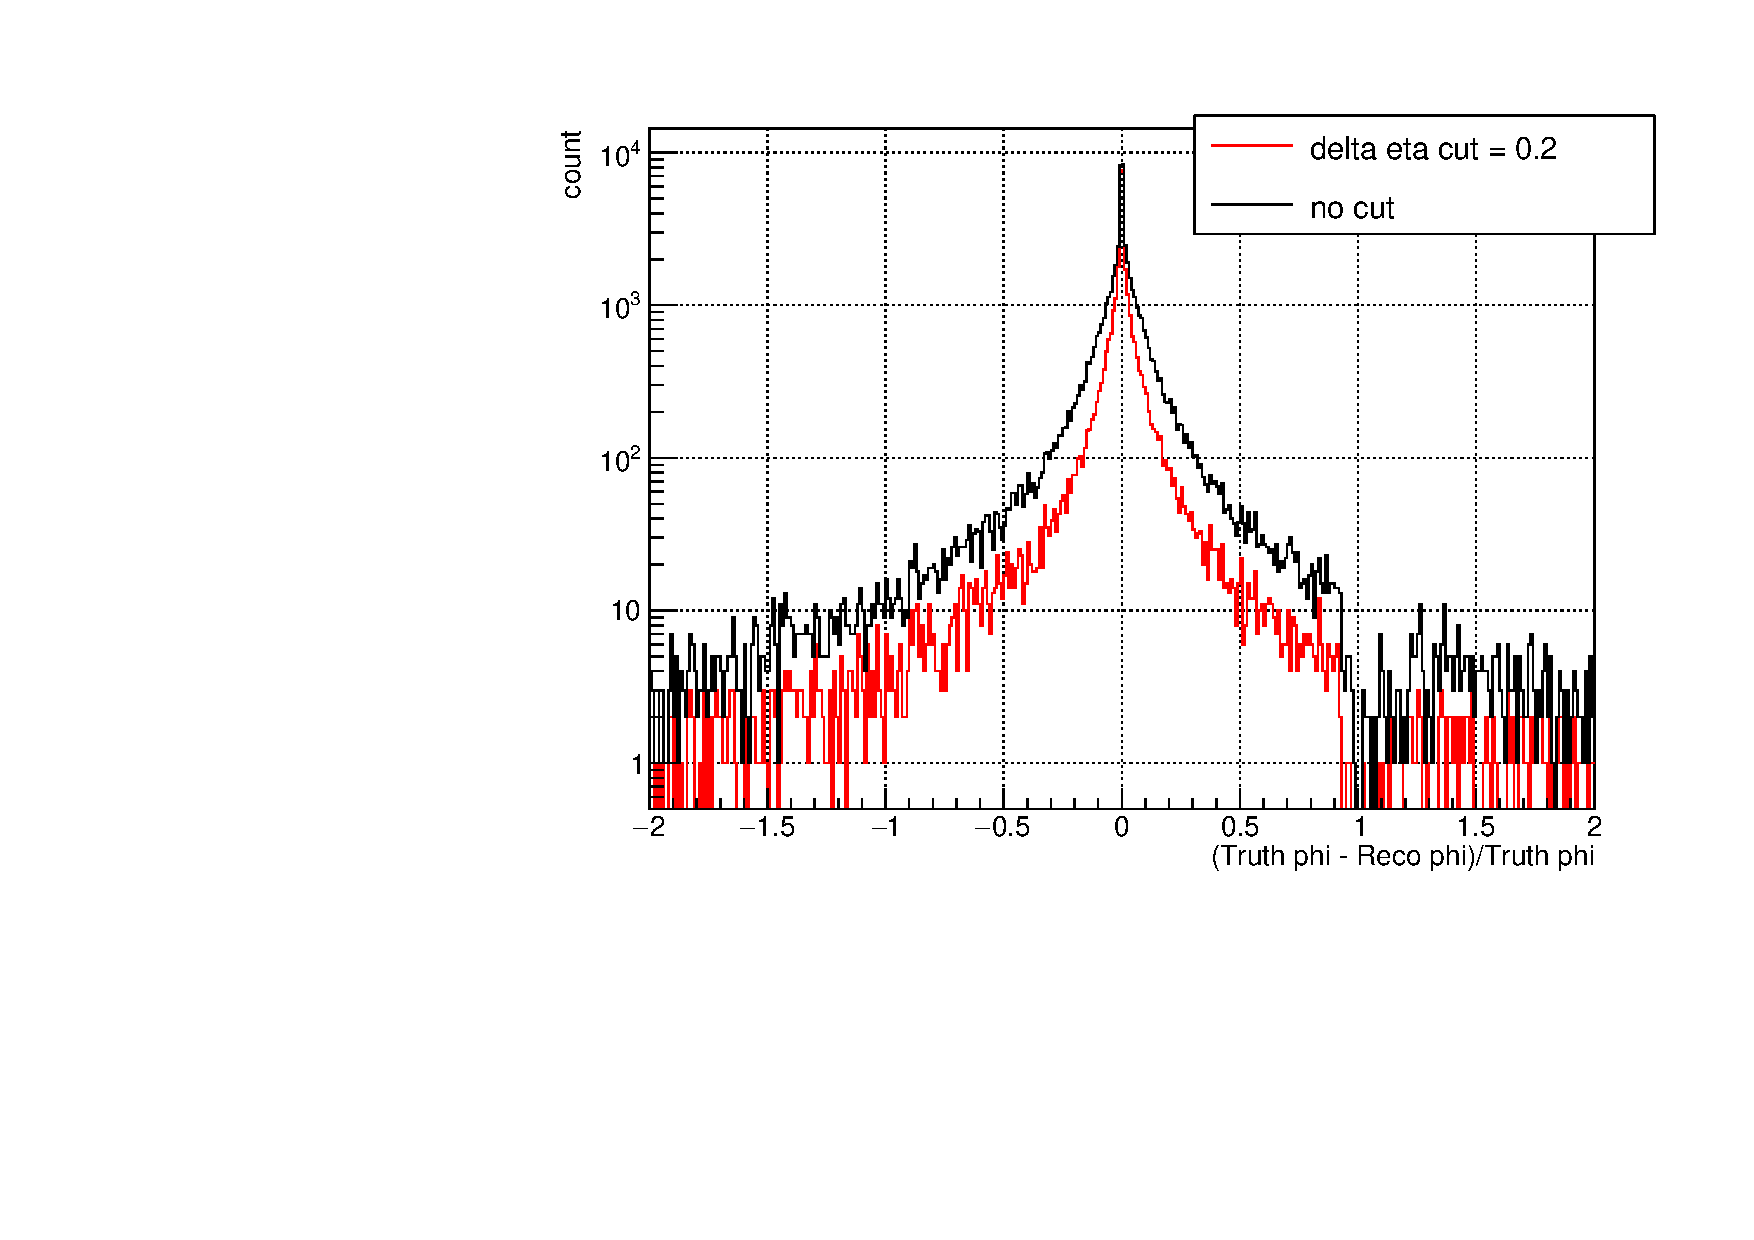
\includegraphics[width=\textwidth]{fig/3_3_phi_resolution.pdf} % Right image
                        \caption{MFT-MCH-MID Track cutted $p_T$}
                        \label{Analysis:Matching:phi resolution}
                    \end{minipage}
                \end{figure}
                The horizontal axis shows the difference between the reconstructed values and the true values, divided by the true values, while the vertical axis represents the number of occurrences. The black histogram represents the resolution without applying the $\Delta \eta$ cut, and the red histogram represents the tracks after applying the $\Delta \eta < 0.2$ cut. By comparing the black and red histograms, we can see that all distributions show improved resolution for single muons.% Furthermore, efficiency and matching purity are provided below.
                % \begin{figure}[htbp]
                %    \centering
                %    \begin{minipage}{0.45\textwidth}
                %        \centering
                %        \includegraphics[width=\textwidth]{fig/3_6_efficiency_pt.pdf}
                %        \captionsetup{labelformat=empty}
                %        \caption{}
                %    \end{minipage}
                %    \hfill
                %    \begin{minipage}{0.45\textwidth}
                %       \centering
                %        \includegraphics[width=\textwidth]{fig/3_6_efficiency_eta.pdf}
                %        \captionsetup{labelformat=empty}
                %        \caption{}
                %    \end{minipage}
                %    \\
                %    \vspace{1em}
                %    \begin{minipage}{0.45\textwidth}
                %       \centering
                    %       \includegraphics[width=\textwidth]{fig/3_6_purity_pt.pdf}
                %        \captionsetup{labelformat=empty}
                %        \caption{}
                %    \end{minipage}
                %    \hfill
                %    \begin{minipage}{0.45\textwidth}
                %        \centering
                %        \includegraphics[width=\textwidth]{fig/3_6_purity_eta.pdf}
                    %       \captionsetup{labelformat=empty}
                %        \caption{} 
                %    \end{minipage}
                %
                %   \vspace{1em}
                %     \begin{minipage}{0.45\textwidth}
                %         \centering
                %        \includegraphics[width=\textwidth]{fig/3_6_effpuri_pt.pdf}
                %         \captionsetup{labelformat=empty}
                %        \caption{}
                %    \end{minipage}
                %     \hfill
                %     \begin{minipage}{0.45\textwidth}
                %         \centering
                %        \includegraphics[width=\textwidth]{fig/3_6_effpuri_eta.pdf}
                %         \captionsetup{labelformat=empty}
                %         \caption{}
                %     \end{minipage}
                % \end{figure}
        
        
                The chosen cut value ($\Delta \eta < 0.2$) was selected to discard only the fake match tracks while keeping the correct match tracks, so the efficiency is reduced, but the matching purity has improved. The efficiency $\times$ purity value remains almost unchanged before and after the cut.